% mnras_template.tex
%
% LaTeX template for creating an MNRAS paper
%
% v3.0 released 14 May 2015
% (version numbers match those of mnras.cls)
%
% Copyright (C) Royal Astronomical Society 2015
% Authors:
% Keith T. Smith (Royal Astronomical Society)

% Change log
%
% v3.0 May 2015
%    Renamed to match the new package name
%    Version number matches mnras.cls
%    A few minor tweaks to wording
% v1.0 September 2013
%    Beta testing only - never publicly released
%    First version: a simple (ish) template for creating an MNRAS paper

%%%%%%%%%%%%%%%%%%%%%%%%%%%%%%%%%%%%%%%%%%%%%%%%%%
% Basic setup. Most papers should leave these options alone.
\documentclass[a4paper,fleqn,usenatbib]{mnras}

% MNRAS is set in Times font. If you don't have this installed (most LaTeX
% installations will be fine) or prefer the old Computer Modern fonts, comment
% out the following line
\usepackage{newtxtext,newtxmath}
% Depending on your LaTeX fonts installation, you might get better results with one of these:
%\usepackage{mathptmx}
%\usepackage{txfonts}

% Use vector fonts, so it zooms properly in on-screen viewing software
% Don't change these lines unless you know what you are doing
\usepackage[T1]{fontenc}
\usepackage{ae,aecompl}

%%%%% AUTHORS - PLACE YOUR OWN PACKAGES HERE %%%%%

% Only include extra packages if you really need them. Common packages are:
\usepackage{graphicx}	% Including figure files
\usepackage{amsmath}	% Advanced maths commands
\usepackage{amssymb}	% Extra maths symbols
\usepackage[xindy]{glossaries}
\glsdisablehyper
\usepackage{subcaption}
\usepackage{tabularx}
\captionsetup{compatibility=false}
\usepackage[normalem]{ulem}

%%%%%%%%%%%%%%%%%%%%%%%%%%%%%%%%%%%%%%%%%%%%%%%%%%

%%%%% AUTHORS - PLACE YOUR OWN COMMANDS HERE %%%%%

% Please keep new commands to a minimum, and use \newcommand not \def to avoid
% overwriting existing commands. Example:
%\newcommand{\pcm}{\,cm$^{-2}$}	% per cm-squared

\newcommand{\GSF}[1]{\noindent\textcolor{blue}{GSF:#1}}
%comments by Marisa
\newcommand{\cM}[1]{\textcolor{magenta}{ #1 --M}}
%comments by Mayuresh
\newcommand{\cMay}[1]{\textcolor{blue}{ #1 --M}}

%glossary
\newacronym{alfa}{ALFA}{Arecibo L-Band Feed Array}
\newacronym{dm}{DM}{Dispersion Measure}
\newacronym{frb}{FRB}{Fast Radio Burst}
\newacronym{fwhm}{FWHM}{Full-Width at Half-Maximum}
\newacronym{gbt}{GBT}{Greenbank Telescope}
\newacronym{htru}{HTRU}{High-Time Resolution Universe}
\newacronym{if}{IF}{Intermediate Frequency}
\newacronym{igm}{IGM}{Intergalactic Medium}
\newacronym{ism}{ISM}{Interstellar Medium}
\newacronym{ligo}{LIGO}{Laser Interferometer Gravitational-Wave Observatory}
\newacronym{lo}{LO}{Local Oscillator}
\newacronym{nip}{NIP}{Non-image Processing}
\newacronym{pll}{PLL}{Phased-locked Loop}
\newacronym{rfi}{RFI}{Radio-frequency Interference}
\newacronym{rrat}{RRAT}{Rotating Radio Transient}
\newacronym{rm}{RM}{Rotation Measure}
\newacronym{ska}{SKA}{Square Kilometre Array}
\newacronym{sefd}{SEFD}{System Equivalent Flux Density}
\newacronym{snr}{S/N}{Signal-to-Noise Ratio}
\newacronym{sps}{SPS}{Single Pulse Search}
\newacronym{tab}{TAB}{Tied-Array Beam}
\newacronym{vlbi}{VLBI}{Very-Long Baseline Interferometry}
\newacronym{xao}{XAO}{Xinjiang Astronomical Observatory}

%%%%%%%%%%%%%%%%%%%%%%%%%%%%%%%%%%%%%%%%%%%%%%%%%%

% Title of the paper, and the short title which is used in the headers.
% Keep the title short and informative.
%\title[FRB Detections and Verification Tests]{Reporting FRB Detections
%and Verification Tests}
\title[FRB Verification Criteria and Reporting]{FRB Verification Criteria and Reporting}

\author[G. Foster et al.]{
Griffin Foster$^{1,2}$\thanks{E-mail: griffin.foster@physics.ox.ac.uk},
Marisa Geyer$^{3}$,
Aris Karastergiou$^{1}$,
Kaustubh Rajwade$^{4}$, 
\and Mayuresh Surnis$^{5,6}$
\\
% List of institutions
$^{1}$University of Oxford, Sub-Department of Astrophysics, Denys Wilkinson Building, Keble Road, Oxford, OX1 3RH, United Kingdom\\
$^{2}$Department of Astronomy, University of California, Berkeley, 501 Campbell
Hall \#3411, Berkeley, CA, 94720, USA\\
$^{3}$SKA-SA, 3rd Floor, The Park, Park Road, Pinelands, South Africa\\
$^{4}$Jodrell Bank Centre for Astrophysics, University of Manchester, Oxford Road, Manchester M13 9PL, United Kingdom\\
$^{5}$Department of Physics and Astronomy, West Virginia University, Morgantown, WV 26505, USA\\
$^{6}$Center for Gravitational Waves and Cosmology, West Virginia University, Chestnut Ridge Research Building, Morgantown,\\ WV 26505, USA\\
}

% These dates will be filled out by the publisher
\date{Accepted XXX. Received YYY; in original ZZZ}

% Enter the current year, for the copyright statements etc.
\pubyear{2018}

% Don't change these lines
\begin{document}
\label{firstpage}
\pagerange{\pageref{firstpage}--\pageref{lastpage}}
\maketitle

% Abstract of the paper
\begin{abstract}
% What is the point of the paper?
% What is the context of the study? What background information is necessary to understand the study?
% How was the study done?
% What is the main take away message?
% What can be said about these results, and how does this affect future work?
The one-off nature of most Fast Radio Bursts (FRBs) necessitates extra scrutiny when
reporting such detections as astrophysical.  The prototypical FRB is a broadband
signal, that occurs over the extent of the receiver frequency range, is
narrow-in-time, and highly dispersed, following a $\nu^{-2}$ relation.  However,
some FRBs appear band-limited, and show apparent scintillation, complex
frequency-dependent structure, or multi-component pulse shapes.  In a search for
rare signals in a noisy data set, the number of false-positive detections is
based on detection thresholds and signal filters.  Such searches should find a
number of false-positive events.  We present examples of false-positive events
that occur in multiple searches, which on initial inspection appear to be
FRB-like, but are found to be due to instrumental variations, noise, and
radio-frequency interference.  Differentiating these false-positive detections
from astrophysical events, requires knowledge and tests beyond performing a
thresholded single-pulse detection.  We discuss post-detection analyses,
verification tests, and data sets which should be provided when reporting an FRB
detection.
\end{abstract}

% Select between one and six entries from the list of approved keywords.
% Don't make up new ones.
\begin{keywords}
radio continuum: transients -- methods: observational
\end{keywords}

%%%%%%%%%%%%%%%%% BODY OF PAPER %%%%%%%%%%%%%%%%%%

\section{Introduction}
\label{sec:intro}

% NOTE: moved here to force the figure higher up in the text
\begin{figure*}
    \centering
    % watermark:terrestrial-frb-letter/notebooks/ALFABURST_events.ipynb
    \begin{subfigure}[t]{0.45\textwidth}
        \centering\captionsetup{width=.95\linewidth}
        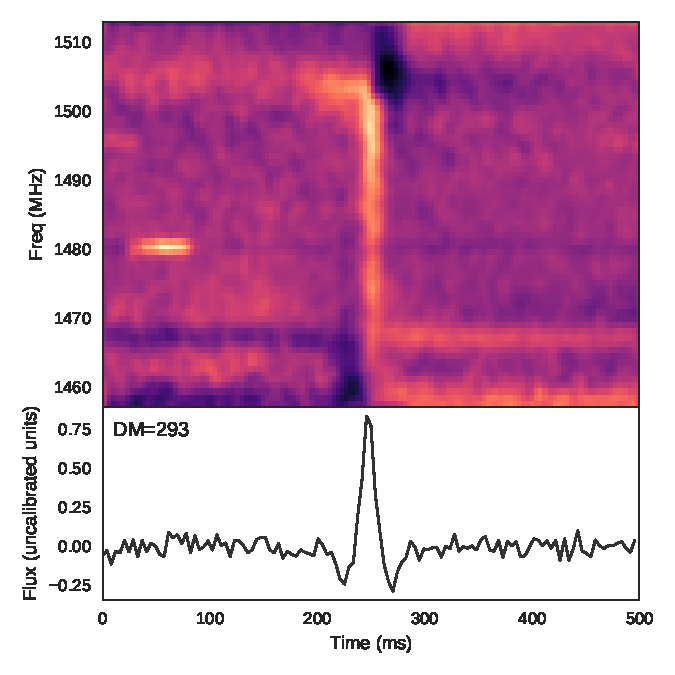
\includegraphics[width=1.0\textwidth]{figures/D20161204_buf23_Beam0.pdf}
        \caption{Detected FRB-like event in Beam 0 of ALFA. The characteristic
        dip before and after the event is due to zero-DM removal which is part
        of the ALFABURST RFI exciser. The strong, narrow band source at 1480~MHz
        around 100~ms is due to a local RFI source.}
        \label{fig:beam0_dynamic_spec}
    \end{subfigure}
    % watermark:terrestrial-frb-letter/notebooks/ALFABURST_events.ipynb
    \begin{subfigure}[t]{0.45\textwidth}
        \centering\captionsetup{width=.95\linewidth}
        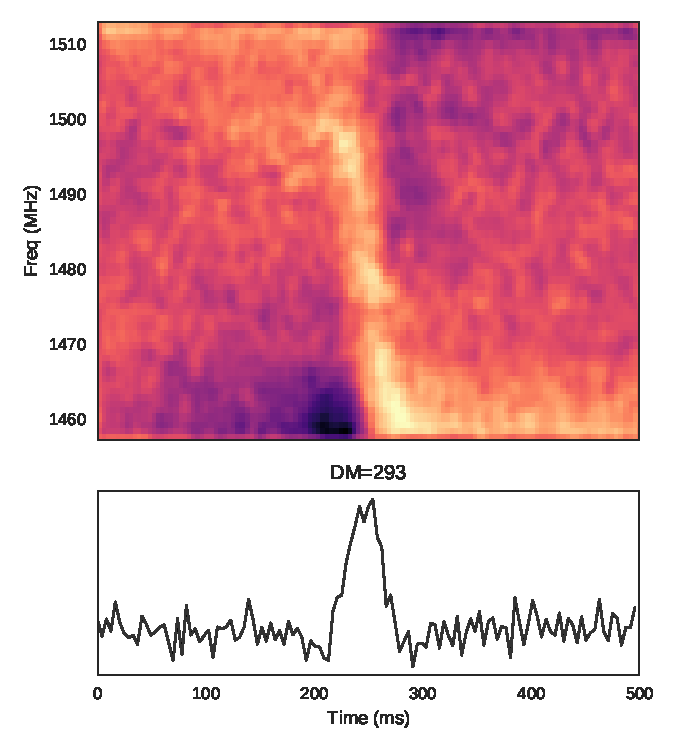
\includegraphics[width=1.0\textwidth]{figures/D20161204_buf4_Beam5.pdf}
        \caption{Detected FRB-like event in Beam 5 of ALFA. The event width
        appears wider than the Beam 0 event as the zero-DM dips are not as
        prominent.
        }
        \label{fig:beam5_dynamic_spec}
    \end{subfigure}
    \caption{
    Dynamic spectrum (top) and \gls{snr}-maximized de-dispersed time series
    (bottom) of an FRB-like event that was detected simultaneously in Beam 0 and
    5 of the ALFA receiver on December 4, 2016. The dynamic spectrum has been
    bandpass normalized.
    }
    \label{fig:dynamic_spec}
\end{figure*}

The origin of \glspl{frb} continues to be a mystery since they were first
reported \citep{2007Sci...318..777L}. The \gls{dm} associated with the reported
events indicate they occur well beyond our galaxy, possibly at cosmological
distances. They appear to be extremely bright, short duration events -- yet
their emission mechanism is not known.  This consensus has developed from the
reporting of detections with multiple telescopes, at different frequencies,
using different instrumentation. \glspl{frb} are difficult to detect as they
require high-gain telescopes which typically have a small beam size, such that
despite many thousands of observing hours, only a few dozen have been reported
as of this writing \citep{2016PASA...33...45P}.

The prototypical \gls{frb} is broad-band, appearing to be broader than most
receivers used in surveys. The pulse is narrow-in-time, on the order of a few
milliseconds in width, with a single component structure. The pulse is highly
dispersed, following a $\nu^{-2}$ relation and appears to be a one-off event
(only FRB121102 is known to repeat, \citealt{2016Natur.531..202S}). Not all
reported detections appear to follow this prototypical form. Many show complex
frequency-dependent structure and are possibly band-limited. The pulse width
varies due to either the emission process or propagation effects such as
scattering from the \gls{ism} and \gls{igm}.

These rare events are detected by automated GPU-accelerated software pipelines
that extensively search a broad range of trial \glspl{dm}, pulse widths, and
starting times.  The de-dispersed time series is then thresholded -- any
peaks above a minimum \gls{snr} are reported as potential detections. The number
of potential detections is usually overwhelming due to \gls{rfi} and system gain
variations. Initially, potential detections were reviewed manually. But, with
the amount of data acquired in recent surveys, it has become a significant time
effort to do so. Further, our understanding of the expected signal properties
has allowed the development of filters and models to select and prioritize
individual events \citep[e.g.][]{2018MNRAS.474.3847F}.

As these sources are rare and generally appear not to repeat (except FRB121102),
there is an issue of verifiability. There is significant \gls{rfi} detectable at
all radio observatories, and there are known anthropogenic sources that appear
FRB-like \citep{2011ApJ...727...18B}.  Given the significant number of \gls{dm}
trials and high-time resolution of the spectra in a typical survey, there are a
large number of false-positives which pass the automated post-processing
detection thresholds.  This is by design, as we would like to severely limit the
potential for false-negatives (type-II errors) in our detection pipelines by
accepting a number of false-positives (type-I errors).  But, given the large
sampling of the parameter search space it can be difficult, if not impossible to
differentiate between a true, astrophysical \gls{frb} (true-positive) and a
`terrestrial' \gls{frb} (false-positive) due to \gls{rfi}, systematics, or other
local effects. As the survey time increases, the likelihood of detecting such a
false-positive will increase. To counter false detection of `terrestrial'
\glspl{frb}, some verification criteria can be tested when reporting a
detection.

In this paper, we present other examples of FRB-like sources which, after
further investigation, we show to be non-astrophysical. Using these and
previously reported \glspl{frb}, we develop a set of criteria to test detections
against and discuss the data, in addition to the detected dynamic spectrum, that
can be reported to provide a robust statement about an \gls{frb} detection.

\section{False-Positive FRB Detections}
\label{sec:false-pos}

During an \gls{frb} search survey there will be a significant number of
false-positive detections. The rate of these detections is set by the minimum
\gls{snr} threshold, the parameter search space, and the terrestrial environment
of the observatory. We use the term `terrestrial' to encompass multiple effects:
anthropogenic radio signals, variations in the observing system, and natural
signals from within the solar system.

Most potential false-positive events are flagged using filters and classifier
models.  The remaining events are commonly examined by eye as expert human
knowledge appears to be the best way to classify a detection. However, time
constraints do not allow for all events to be classified in this way. On
inspection, true astrophysical events and terrestrial events can be difficult to
differentiate between, even by the expert eye.  These terrestrial events,
indeed, should appear like astrophysical \glspl{frb} as they have passed the
detection pipeline thresholds. 

Studies of the telescope state during detection, can often assist in determining
the origin of an event. Nonetheless, ambiguities can remain, leading to the
precarious nature of reporting an \gls{frb} as astrophysical.  In this section
we present examples of such events -- which on initial inspection appear to be
astrophysical, but after further investigation prove to be terrestrial in
origin.

\subsection{ALFA Terrestrial FRB}
\label{sec:D20161204}

In the two years of the initial ALFABURST survey \citep{2017ApJS..228...21C,
2018MNRAS.474.3847F}, over 200k 8.4-second data windows were recorded in which
the \gls{frb} search pipeline detected events using a minimum \gls{snr}
detection threshold of 10. The vast majority of these events were due to
\gls{rfi} and instrumental variations, while others were due to bright single
pulses of known pulsars.  The classifier model outputs an ordered list of events
based on the likelihood of the event being a pulse.

A narrow-in-time, broad-in-frequency, millisecond pulse was detected with the
ALFABURST system at MJD 57726.563263913 / Unix time 1480858266 (09:31:06 Arecibo
local time on 2016, December 4) in Beam 0 (the central beam) of the \gls{alfa}
receiver\footnote{http://www.naic.edu/alfa/} (Figure
\ref{fig:beam0_dynamic_spec}) which we label as the D20161204 event for this
discussion. ALFABURST was processing 56~MHz of bandwidth between 1457~MHz and
1513~MHz. The \gls{snr} of this pulse is maximized when the pulse is
de-dispersed with a \gls{dm} of 293~pc~cm$^{-3}$, and the 256~$\mu$s time
resolution is decimated by a factor of 16 to a time resolution of 4~ms. The
de-dispersed time series shows an approximately 20~ms \gls{fwhm} pulse.  The dip
before and after the pulse is due to the zero-DM filtering (i.e. the moving
channel average is subtracted) before pulse detection
\citep{2009MNRAS.395..410E}. This is a simple way to remove a drifting gain
baseline at the cost of removing some of the overall pulse power, particularly
at low DM trials.

On initial inspection, this event looks like a promising new astrophysical
\gls{frb}. The flux density of the pulse can be computed using the radiometer
equation,
%
$$
S = \textrm{SEFD} \frac{\textrm{S/N}}{\sqrt{D \; \Delta \tau \;
\Delta \nu}}
$$
%
using a \gls{sefd} of 3~Jy for the \gls{alfa} receiver. This results in a flux
density of \mbox{$S = 66$}~mJy from Beam 0, which would be lower than what is
observed for any previously detected \gls{frb} \citep{2016PASA...33...45P}.
However, this flux estimate is a lower limit, as we are assuming the source is
at the center of the beam. The pulse width is large for an \gls{frb} but within
the range of those previously reported.

Of the six other \gls{alfa} beams, the event only appears in Beam 5 (Figure
\ref{fig:beam5_dynamic_spec}), which is adjacent to Beam 0.  This pulse lines up
with the Beam 0 event in time exactly, but the event \gls{snr} was maximized
($S/N=16$) for a DM of 829~pc~cm$^{-3}$. By testing a range of DM values, we
found that this event appeared to decrease in width for lower DM trials.
\gls{rfi} clipping was applied during this event which is known to introduce a
bias, resulting in a maximized \gls{snr} at a different DM trial.  We thus
conclude that the Beam 0 and Beam 5 event are the same event.

In the immediate period before and after the pulse, there are no similar events
(Figure \ref{fig:dm_time}). The event appears to be isolated in time, with a
fairly compact representation in DM-time space (Figure \ref{fig:dm_time_event})
similar to that of a single pulse from a high DM pulsar, such as PSR B1859+03
(Figure \ref{fig:dm_time_B1859}).

\begin{figure}
    \centering
    % watermark:terrestrial-frb-letter/notebooks/ALFABURST_events.ipynb
    \begin{subfigure}[t]{0.5\textwidth}
        \centering\captionsetup{width=.95\linewidth}
        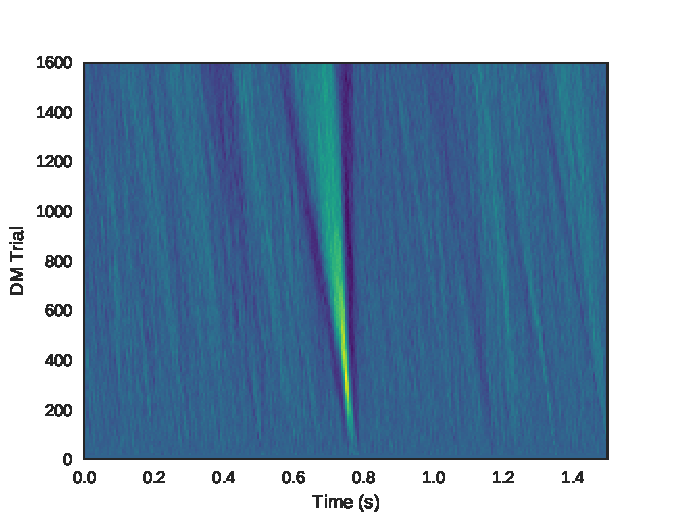
\includegraphics[width=1.0\textwidth]{figures/D20161204_dmtrials_buf23_Beam0.pdf}
        \caption{DM vs. time plot of for a 1.5~second window centred on the
        December 4th event in Beam 0. The \gls{snr} peaks at a DM of
        293~pc~cm$^{-3}$. There is a significant detection at larger DM trials
        due to the width of the pulse.
        }
        \label{fig:dm_time_event}
    \end{subfigure}
    % watermark:terrestrial-frb-letter/notebooks/ALFABURST_events.ipynb
    \begin{subfigure}[t]{0.5\textwidth}
        \centering\captionsetup{width=.95\linewidth}
        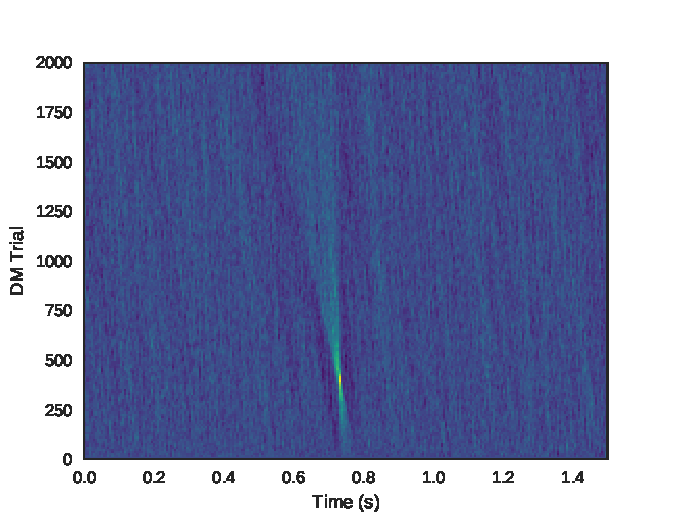
\includegraphics[width=1.0\textwidth]{figures/B1859_dmtrials.pdf}
        \caption{DM vs. time plot of a bright single pulse from PSR B1859+03
        which has a DM of 402~pc~cm$^{-3}$ and pulse width of 11~ms (W50).
        }
        \label{fig:dm_time_B1859}
    \end{subfigure}
    \caption{DM-space plot shows the characteristic butterfly pattern of the
    narrow-in-time, dispersed pulse detected by ALFABURST. A single pulse
    detection of PSR B1859+03 is shown for reference.
    }
    \label{fig:dm_time}
\end{figure}

The telescope was pointed at a fixed Dec (+15:11:28.34) and drifting in RA
(event detected at RA=14:42:26.18), i.e. a fixed (alt, az)-pointing during the
event. No known pulsar or \gls{rrat} with a similar DM lies within the beam
primary lobe of this pointing.

The telescope logs provide the first indication that this event is due to a
local source. As ALFABURST is a commensal observation survey the search pipeline
regularly checks the status of the receiver turret and the \gls{if}. \gls{alfa}
was logged as active and the \gls{if} remained unchanged during this time, but
the turret was in a different position than where ALFA should be if it were at
the secondary focus.

The observing schedule for the morning of December~4, was project
P3080\footnote{http://www.naic.edu/vscience/schedule/tpfiles/MichillitagP3080tp.pdf}
using \gls{alfa} to perform an \gls{frb} survey of the Virgo cluster until 09:00
local time, followed by Project
R3037\footnote{http://www.naic.edu/vscience/schedule/tpfiles/TaylortagR3037tp.pdf},
an S-Band RADAR observation.  The event occurred during a time of no active
observation with \gls{alfa} active but in the wrong turret position.

The average bandpass of Beam 0 and Beam 5 during the time of the event shows
that the shape and system noise appear different to what is expected during
typical observations (Figure \ref{fig:bandpass_response}).  Beam 0 and 5
bandpasses appear similar and have overlapping narrow-band RFI features during
the recorded time window.  The system noise appears to be higher during the
event, which leads to smoother bandpasses than what is typical.  In the
detection pipeline the data are normalized, which removes all absolute scaling in
the process. This indicates that the \gls{sefd} is too low in our flux
calibration.  This increase in system noise is due to the change in turret
position, causing the \gls{alfa} feed to pick up reflections from other
equipment in the dome, and the dome as a warm source.  This event is most likely
due to the analogue electronics becoming non-linear from this increase in system
noise.

% watermark:terrestrial-frb-letter/notebooks/ALFABURST_events.ipynb
\begin{figure}
    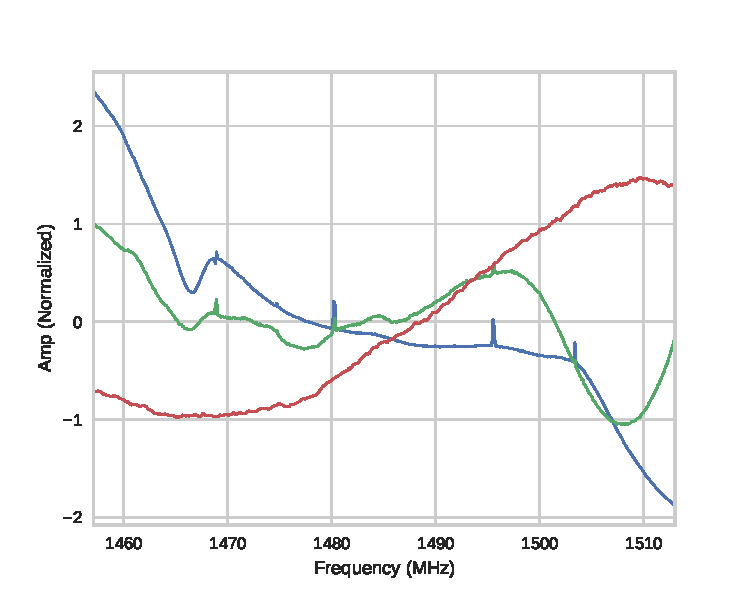
\includegraphics[width=1.0\linewidth]{figures/bandpass_response.pdf}
    \caption{Average bandpass response during the December 4, 2016 event for
    Beam 0 (green) and Beam 5 (blue). A typical bandpass (red) is plotted for
    reference. These bandpasses have been normalized in the detection pipeline.
    }
    \label{fig:bandpass_response}
\end{figure}

Evidence for analogue gain variations is further justified by considering the
data over a larger time window.  Approximately 80 seconds before the event,
large structures across the band are present (Figure
\ref{fig:beam0_dynamic_spec_80s}). Though not as narrow-in-time as the event,
they appear related to the same phenomenon.  The DM$-$time plot (Figure
\ref{fig:beam0_dmtrials_80s}) shows that much of the structure would be detected
as dispersed pulses.  In particular, the structure around 4 seconds would be
detected as a wide-in-time, highly dispersed pulse.  And the structure
immediately proceeding it would be detected as a negatively dispersed pulse.  We
do not detect these as pulses because we have limited our search space to
narrow-in-time width pulses and positive \glspl{dm}.

\begin{figure*}
    \centering
    % watermark:terrestrial-frb-letter/notebooks/ALFABURST_events.ipynb
    \begin{subfigure}[t]{1.0\textwidth}
        \centering\captionsetup{width=.95\linewidth}
        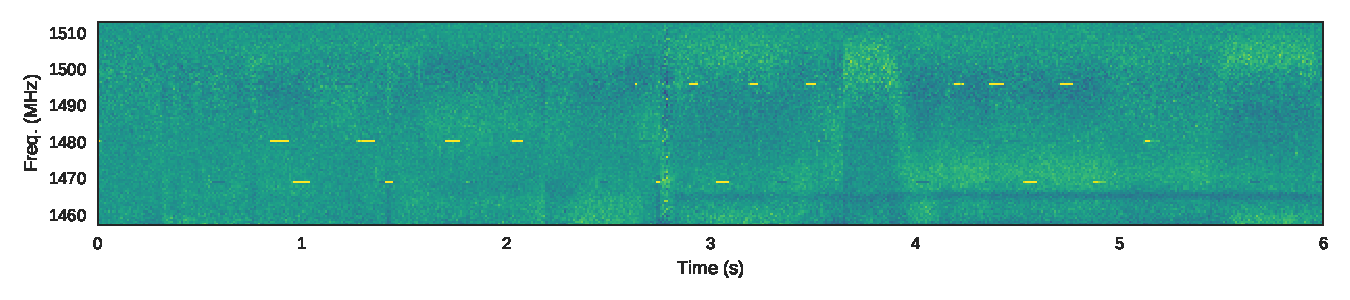
\includegraphics[width=1.0\textwidth]{figures/D20161204_spect_buf21_Beam0.pdf}
        \caption{Dynamic spectrum shows frequency evolution of the bandpass as a
        function of time with structures similar to the D20161204 event.
        }
        \label{fig:beam0_dynamic_spec_80s}
    \end{subfigure}
    % watermark:terrestrial-frb-letter/notebooks/ALFABURST_events.ipynb
    \begin{subfigure}[t]{1.0\textwidth}
        \centering\captionsetup{width=.95\linewidth}
        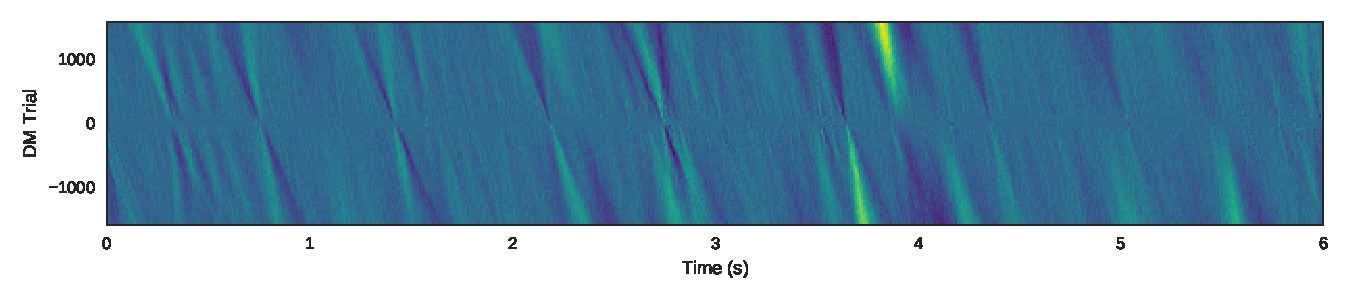
\includegraphics[width=1.0\textwidth]{figures/D20161204_dmtrials_buf21_Beam0.pdf}
        \caption{DM trials from -1600 to 1600 show that there would be both
        positive and negative pulse detections during this time window.
        }
        \label{fig:beam0_dmtrials_80s}
    \end{subfigure}
    \caption{Dynamic spectrum (top) and DM-time plot (bottom) of 6 seconds from
    beam 0 approximately 80 seconds before the D20161204 event.
    }
    \label{fig:beamo0_80s}
\end{figure*}

In isolation, and taking into account the one-off, transient nature of FRBs, the
initial Beam 0 detection reasonably appear to be astrophysical. But, after
studying the telescope state and examining data across a larger time window
(several seconds) around the event, we can confidently classify this event as
terrestrial.

\subsection{Low-S/N False-Positive Detections}
\label{sec:low_snr}

While the D20161204 event (Section \ref{sec:D20161204}) is a rare false-positive
detection based on a unique telescope state, other false-positive events occur
regularly.  As automated search pipelines are set up to carry out an extensive
search in trial \glspl{dm}, pulse width, and starting time, it is reasonable to
expect a large number of low-\gls{snr} false-positive detections. A minimum
\gls{snr} cut-off (usually 6-10) is set to limit the number of these
false-positives.

For example, on July 30, 2015 an apparently 10-$\sigma$ event with a DM of
1370~pc~cm$^{-3}$ was detected (Figure \ref{fig:D20150730}) by the ALFABURST
pipeline in Beam 5. The pulse can barely be seen in the dynamic spectrum, but in
the DM-time plot, there is a compact peak centred at a DM of 1370~pc~cm$^{-3}$
with no other similar events apparent.  After re-analysis of the dynamic
spectrum noise, this event only has an \gls{snr}$\sim$6, but was reported as a
higher \gls{snr} because of the data window size used to calculate the system
noise.  Locally in time, there is an increase in system noise, leading to a
reduced \gls{snr}.  This is not an uncommon event and many of these events have
no immediate explanation.

% watermark:terrestrial-frb-letter/notebooks/ALFABURST_events.ipynb
\begin{figure}
    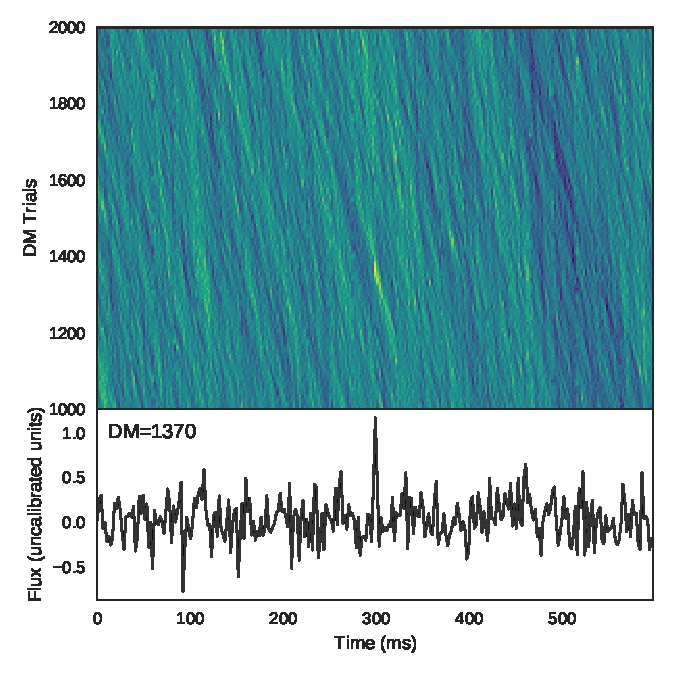
\includegraphics[width=1.0\linewidth]{figures/D20150730_buf23_Beam6_dmtrial.pdf}
    \caption{DM-space plot and time series of a high DM event with reported
    \gls{snr} above 10-$\sigma$ on July 30, 2015. After re-analysis and review
    of the telescope meta-data it was determined that this event was due to
    local system noise.
    }
    \label{fig:D20150730}
\end{figure}

These types of events prove to be difficult to validate as either astrophysical
or terrestrial if sufficient data are not recorded during a detection, providing
with an evidence to be confident about the event's origin. The choice of minimum
\gls{snr} is set based on the willingness of the observers to sort through
false-positive events.  There are likely many low-\gls{snr} \glspl{frb} that are
labelled as false-positive events.  The reported detection of a pulse from
FRB121102 with APERTIF \citep{atel10693} had an \gls{snr}$\approx 4$. In a blind
survey across different sky positions and trial \glspl{dm}, this would not be a
significant detection.  But, the sky position and \gls{snr}-maximized DM of the
repeating FRB121102 is known, thus a lower \gls{snr} detection may be reasonable
to report.  We usually require a large \gls{snr} to validate a detection.  As
the parameter space (trial \glspl{dm}, pulse width range) and number of
observations grow we expect to see an increase in the number of high-\gls{snr},
false-positive events.

\subsection{ARTEMIS RADAR Detection}
\label{sec:LOFAR_RADAR}

ARTEMIS \citep{2015MNRAS.452.1254K} is a low-frequency \gls{frb} search survey
run on the LOFAR-UK station at the Chilbolton Observatory.  The survey uses a
similar fractional bandwidth ($\sim 0.04$) to ALFABURST, but is centred at
145~MHz.  In this survey, known pulsars regularly transit the beams that are
fixed in local coordinates, and single pulses are routinely observed.  An
\gls{rfi} exciser has been developed for this survey that successfully removes
the majority of false-positive events. Over many thousands of observing hours,
rare events occasionally pass this filter.

A particularly interesting event for which the \gls{snr} was maximized at a
\gls{dm} of 85~pc~cm$^{-3}$ is shown in Figure \ref{fig:lofar_dynamic}. Though
this event has a low DM compared to the reported \glspl{frb}, this still proves
to be a relevant example as discussed later in this section.  The narrow-in-time
pulse can be seen in the dynamic spectrum at frequencies above 146 MHz, but not
at lower frequencies where it could be hidden by narrow band \gls{rfi}.  The
de-dispersed time series shows a high-\gls{snr} detection of a pulse of
approximately 20~ms in width.  The beam pointing during the time of the event is
not associated with any known pulsar or RRAT around a DM$\sim$85~pc~cm$^{-3}$.

% watermark:terrestrial-frb-letter/notebooks/LOFAR_RADAR.ipynb
\begin{figure}
    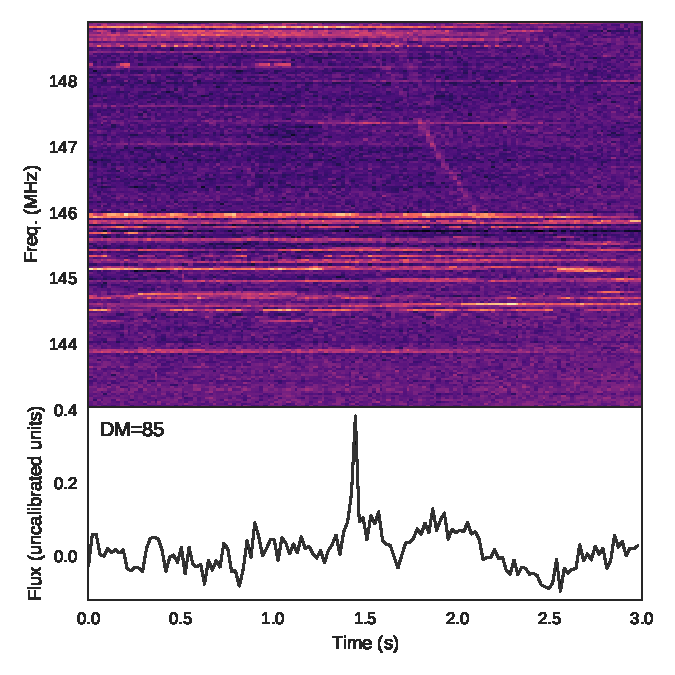
\includegraphics[width=1.0\linewidth]{figures/LOFAR_dynamic.pdf}
    \caption{A dispersed pulse detected by the automated ARTEMIS search pipeline
    at the LOFAR-UK station. The \gls{snr} is maximized when the signal is
    dedispersed to a DM of 85~pc~cm$^{-3}$. The dynamic spectrum has a time
    resolution of 20~ms and frequency resolution of 3~kHz.
    }
    \label{fig:lofar_dynamic}
\end{figure}

Plotting the event in DM-time space across the ARTEMIS DM range
($0-320$~pc~cm$^{-3}$, Figure \ref{fig:lofar_dm_time}) shows a strong, compact
detection as expected of a dispersed pulse. But, the apparent limited bandwidth
of the pulse means that the pulse does not necessarily follow a $\nu^{-2}$
dispersion relation. For example, with a limited fractional bandwidth a linearly
dispersed pulse can be approximately modelled with such a relation.

% watermark:terrestrial-frb-letter/notebooks/LOFAR_RADAR.ipynb
\begin{figure}
    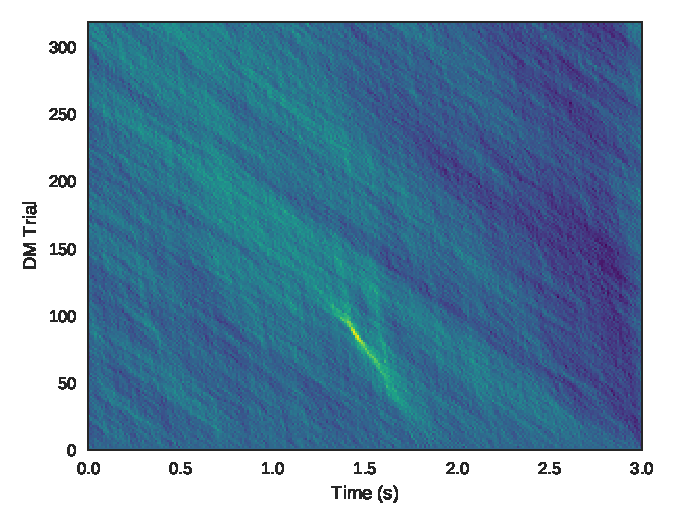
\includegraphics[width=1.0\linewidth]{figures/LOFAR_dm_time.pdf}
    \caption{DM-space plot over the DM trial range of the ARTEMIS survey. A
    strong, compact detection occurs at a DM of 85~pc~cm$^{-3}$ with no other
    apparent events during the time.
    }
    \label{fig:lofar_dm_time}
\end{figure}

The ARTEMIS search pipeline, like most \gls{frb} search pipelines, decimates the
dynamic spectrum in time to search over a range of pulse widths. The \gls{snr}
of the event shown in Figure \ref{fig:lofar_dynamic} is maximized for a time
decimation factor of 64. With a native resolution of $327.68~\mu s$, this
results in a decimated time resolution of 20~ms. At this resolution, the pulse
appears to be a continuous broadband pulse. When an event is detected in the
pipeline, the un-decimated dynamic spectrum is saved. Plotting at 1~ms time
resolution (Figure \ref{fig:lofar_dynamic_high}), the repeating nature of a
linear frequency-modulated signal used for pulse compression in RADAR can be
seen.

% watermark:terrestrial-frb-letter/notebooks/LOFAR_RADAR.ipynb
\begin{figure}
    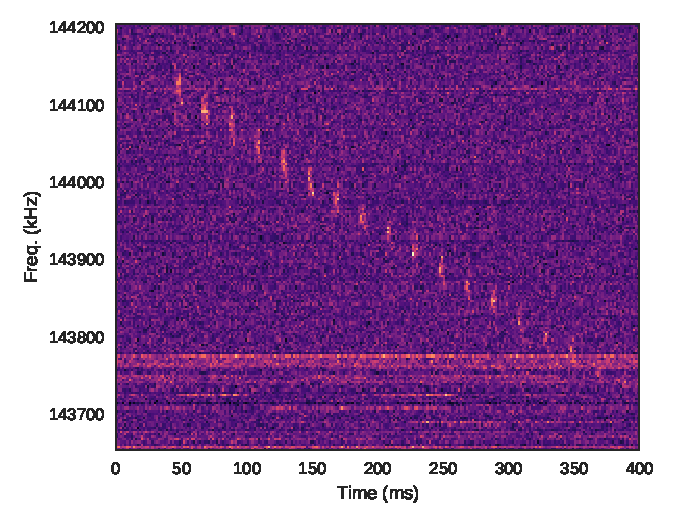
\includegraphics[width=1.0\linewidth]{figures/LOFAR_dynamic_high_res.pdf}
    \caption{A zoomed in view of the event in Figure \ref{fig:lofar_dynamic} at
    high time (1~ms) and frequency (1.5~kHz) resolution shows the distinct
    pattern of a linear frequency-modulated RADAR pulse.
    }
    \label{fig:lofar_dynamic_high}
\end{figure}

In RADAR observations, the bandwidth of the transmitter provides information on
the range and direction of a target. A narrow-band RADAR transmitter can be used
to approximate a larger bandwidth by modulating the frequency of the transmitted
pulse. The narrow-band (in frequency) pulse is stepped in frequency across a
transmission band. Between each step the pulse is not transmitted, resulting in
the gaps in time between pulses, such as in Figure~\ref{fig:lofar_dynamic_high}.
An increase in the delay between the narrow-band pulses will result in a
wide-band pulse that appears more dispersed.

Linear frequency-modulation is the most typical form of chirp compression, but
non-linear methods are also used. Such a modulation technique may be the origin
of the detections in the next section.  There are a number of allocated RADAR
usages in the LOFAR observing band which could be the source of the observed
RADAR pulse \citep{ofcom2017}.  RADAR is used from UHF to C-band, covering a
wide range of frequencies at which \gls{frb} surveys operate. We could not
determine the exact origin of the RADAR pulse, since RADAR is used for
commercial and military purposes, most of these signal specifications,
modulations, and source locations are proprietary.

As the RADAR signal is a dispersed pulse, we expect to detect such signals with
\gls{frb} pipelines.  Verification of this event is straightforward when the
high-time and frequency resolution data are available to reveal the narrow-band,
pulsed nature of the event.

\subsection{XAO Repeating Event}
\label{sec:xao_event}

% Likely answer:
% RADAR for tracking a space re-entry
% repeating nature to keep constant track
% once-off nature means it happened only once
% Jiuquan Satellite Launch Center not far from XAO.
% shenzhou 11 landed in inner mongolia on november 2018, around 2:15 pm china
% time
% first pulse: 2016-11-18 02:24:24.958 UTC
% last pulse: 2016-11-18 03:31:56.592 UTC
% china time is +8 UTC
% https://en.wikipedia.org/wiki/Shenzhou_11
% https://spaceflight101.com/shenzhou-11-undocking-set-for-landing/
%
% http://www.radartutorial.eu/01.basics/Distance-determination.en.html
% http://www.radartutorial.eu/08.transmitters/Intrapulse%20Modulation.en.html

The 25-m Nanshan Telescope at \gls{xao} is currently running an FRB survey which
covers over 300~MHz at L-band, sampling at $64 \; \mu s$ resolution. On November
18, 2016 hundreds of bright, dispersed pulses were detected. The pulses varied
in \gls{snr}, but had the same \gls{snr}-maximized DM of 531.8~pc~cm$^{-3}$. The
pulses show a distinct double peak (each peak $\sim 2$~ms wide) separated by
$\sim 3$~ms (Figure \ref{fig:xao_dynamic}). The pulses are only apparent in a
portion of the band.

% watermark:/home/griffin/data/XAO/coadd_pulses.ipynb
\begin{figure}
    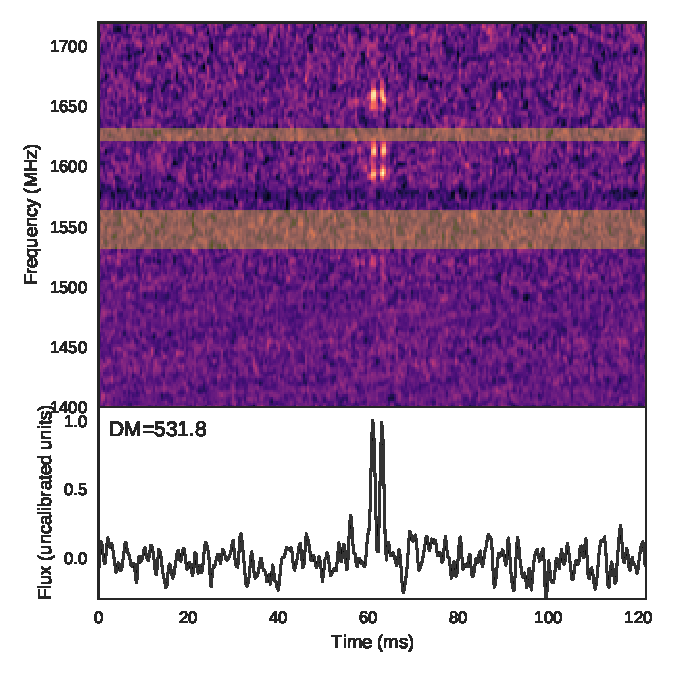
\includegraphics[width=1.0\linewidth]{figures/XAO_pulse_dynamic.pdf}
    \caption{Example of a detected pulse with the Nanshan Radio Telescope at XAO
    which is \gls{snr} maximized at a \gls{dm} of $531.8$~pc~cm$^{-3}$.
    Hundreds of such pulses were detected over a period of a few hours. The
    orange bars represent regions that have had significant constant-in-time
    \gls{rfi} replaced by noise.
    }
    \label{fig:xao_dynamic}
\end{figure}

A periodicity search revealed a periodicity of $\sim 1.7$~s, but the residuals
were orders of magnitude higher than that of a typical pulsar periodicity
search.  Further, the pulses were seen at different pointings across the sky.
Most were detected at a low altitude pointing angle, but some were detected
close to zenith.  This rules out a pulsar, or an astronomical source in general.

Figure \ref{fig:xao_summed} shows the sum of the de-dispersed (using a DM of
531.8~pc~cm$^{-3}$) phase-aligned pulses.  This `folded' spectrum shows an
S-shaped broadband pulse which covers most of the observing band. There is also
regular, narrow-band frequency modulation ($\sim4$~MHz) in the pulse structure.
The structure is likely due to non-linear frequency modulation, used in
chirped RADAR systems, similar to the linear frequency-modulated signal observed
in Section \ref{sec:LOFAR_RADAR}.

% watermark:/home/griffin/data/XAO/coadd_pulses.ipynb
\begin{figure}
    \includegraphics[width=1.0\linewidth]{figures/XAO_summed_dynamic.pdf}
    \caption{The `folded' dynamic spectrum of 182 high-\gls{snr} pulses detected
    with the Nanshan Radio Telescope.  The low-level, non-linear frequency
    modulation can be seen across the band. The orange bars represent regions
    that have had significant constant-in-time \gls{rfi} replaced by noise.
    }
    \label{fig:xao_summed}
\end{figure}

A thorough search of possible local sources, such as new equipment, vehicles,
and aircraft was preformed, with no obvious candidate being found. Detection of
multiple pulses at different beam pointings indicates the source may be directly
illuminating the feed. The source is likely not due to system electronics
because of the complex frequency modulation but rather due to a local
transmitter.

The Nanshan L-band receiver is a single pixel system. It could be that a
multi-beam system such as the Parkes Multi-beam or ALFA would detect these
events in many of the beams, and the event could be classified as terrestrial.

Had only a single pulse been detected, for example if the source was weaker, or
the telescope was only sensitive to the highest \gls{snr} event, it would be
difficult to show that the event was due to \gls{rfi}.  Multiple reported
\glspl{frb}, including the repeater FRB121102, do not cover the entire observing
band. This has been explained by various intrinsic or intermediate effects
(scintillation, plasma lensing). In the case of a single detected pulse, it would
be reasonable to report it as an astronomical \gls{frb}.

A dispersion relation parameter estimation of the individual pulses was found to
deviate from a $\nu^{-2}$ relation by $1.5 \sigma$. A dispersed astrophysical
source should always follow a cold plasma $\nu^{-2}$ relation. As shown, sources
which approximately fit this relation will still be detected with de-dispersion
algorithms.

The \gls{snr}-maximized DM of the XAO events is due to the frequency structure
of the pulse, but also the receiver system.  Knowing the broadband structure of
the source, we can build a simple model to show that a non-linear modulation
scheme can produce a range of apparent \gls{snr}-maximized events depending on
the observing band compared to the pulse transmission band.

The pulse can be modelled using a logistic function which covers a bandwidth
from $\nu_{\textrm{p,0}} = 1350$~MHz to $\nu_{\textrm{p,1}} = 1750$~MHz (Figure
\ref{fig:xao_simulation_diagram}). The time duration of the pulse $\Delta
t_{\textrm{pulse}}$ is fixed such that central frequency range of the pulse has
an \gls{snr}-maximized DM of approximately 530~pc~cm$^{-3}$. The pulse is given
a width ($\Delta t_{\textrm{width}}$) by convolving the logistic function with a
3~ms wide Gaussian. The amplitude of the pulse is set to unity across the extent
of the band.

% figures/simulation_digram.odg
\begin{figure}
    \includegraphics[width=1.0\linewidth]{figures/simulation_diagram.pdf}
    \caption{Non-linearly modulated pulse (logistic function) and receiver model
    used to simulate the response and \gls{snr}-maximized DM fit to a pulse
    similar to the one detected at XAO.
    }
    \label{fig:xao_simulation_diagram}
\end{figure}

A receiver model is used to simulate the observation. This model is
parameterized by a central observing frequency $\nu_{\textrm{obs,c}}$, bandwidth
$\Delta \nu_{\textrm{obs}}$, number of observing frequency channels
$n_{\textrm{freqs}}$, and per channel noise $\sigma_{\textrm{chan}}$. The
bandpass is modelled as a Gaussian.

% watermark:/home/griffin/data/XAO/Non-Linear-Pulse-Simulation.ipynb
\begin{figure}
    \includegraphics[width=1.0\linewidth]{figures/simulatedRADARdm.pdf}
    \caption{\gls{snr}-maximized DM trials for a simulation of the XAO
    non-linearly modulated pulse centred at 1550~MHz over a range of central
    observing frequencies, and receiver bandwidths.
    }
    \label{fig:xao_simulated_dm}
\end{figure}

Detection of the pulse is simulated across a range of central observing
frequencies and receiver bandwidths (Figure \ref{fig:xao_simulated_dm}). The
\gls{snr}-maximized DM is determined by performing a trial DM search from 0 to
4000~pc~cm$^{-3}$ in integer increments.  For all bandwidths, when the central
observing frequency is near the centre of the pulse the apparent DM of
$\sim530$~pc~cm$^{-3}$ maximizes the detection \gls{snr}. However, when the
central observing frequency is shifted relative to the pulse centre frequency a
range of \gls{snr}-maximized \glspl{dm} are reported, depending on the receiver
bandwidth. This model can be used to approximate an astrophysical \gls{frb}
signal at any frequency and bandwidth for a given receiver.

Since the initial detection of the pulses in November 2016 the pulses have not
been re-detected. While the source is terrestrial in origin, these pulses
present a situation where terrestrial sources can easily be misidentified as
one-off astronomical events. This event, along with the other events presented
in this section should present a case for developing common criteria, observing
strategies, and data recording to improve the confidence in \gls{frb}
detections.

\section{FRB Verification}
\label{sec:verify_crit}

Our ability to discover \glspl{frb} depends on how well we can describe what an
FRB is, and on having available the data to search for and verify events. There is currently no formal definition, rather a set of community
standards. These vary between groups and instruments, but usually include
information drawn from images of power in the time-frequency plane and the
time-DM plane, information about the telescope state, information related to the
presence of the signal in one or more beams.  These standards are set in order
to compare each new detection to an \gls{frb} archetype: a broad band signal,
excessively dispersed for its Galactic line of sight, following a $\nu^{-2}$
dispersion relation, and narrow in pulse width, such as FRB130626
\citep{2016MNRAS.460L..30C} (Figure \ref{fig:FRB130626}). This process of
comparison follows the prototype theory of categorization \citep{ROSCH1976382}
which suggests that certain examples of a category are more prototypical than
others. A category will contain examples which deviate from the prototypical as
the prototype is an exaggeration of features deemed characteristic to the
category.

% FRB130626
% aslxlap07:/local/griffin/data/FRB/FRB130626/FRB130626.ipynb
\begin{figure}
    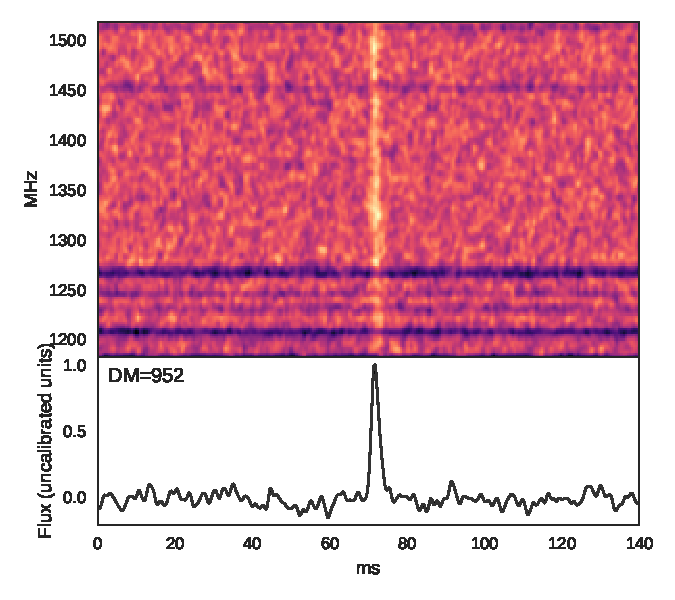
\includegraphics[width=1.0\linewidth]{figures/FRB130626.pdf}
    \caption{FRB130626 is a prototypical FRB with a broad-in-frequency,
    narrow-in-time, single component pulse at a DM=952~pc~cm$^{-3}$ well in
    excess of the Galactic DM contribution in that line of sight.
    }
    \label{fig:FRB130626}
\end{figure}
\subsection{Data}
%\section{Detection Reporting}
\label{sec:detect_report}

The one-off nature of \glspl{frb} makes it essential to do sufficient
due-diligence when reporting on a detection or triggering a follow-up
observation to verify a true-positive detection. Over the past decade of
\gls{frb} surveys a number of techniques have been developed to efficiently
filter the total power, time-frequency data for dispersed pulses. Additional and important tests require capturing more data. It is not always possible to capture sufficient data for every desired test, nor is it possible with every observational setup.  The effort is, however, justified, as questioning a detection from many possible angles will lead to higher confidence in reporting an event as astrophysical or rejecting it as not interesting. 

If most \glspl{frb} are indeed one-off events, then the detection data are the
only data that will be available. Publication of the detection data allow independent
verification, and can be used as input to test independent
pipelines. The following should at least be available:

\begin{enumerate}
    \item A dynamic spectrum which fully encompasses the extent of the dispersed
    pulse. Preferably, both the raw dynamic spectrum and the \gls{rfi} flagged
    and/or normalized spectrum computed in the detection pipeline would be available.
    \item Technical data such as time and frequency information, telescope pointing, and other telescope
    observing parameters.
    \item For a multi-beam system, dynamic spectra of each beam covering the
    extent of the pulse. Similarly for a \gls{tab} or interferometric detection.
    \item The detection parameters such as peak \gls{snr}, best DM, pulse width, and others.
    \item A list (or guide) of software (including the versions) and parameters used
    to generate diagnostic plots.
\end{enumerate}

These requirements are typically met in previously reported \gls{frb}
detections. Often the public data have been normalized, which is useful
for studying the event but can hide instrumental effects.  The last point,
a guide on which software was used is often not reported.  Differences in
software and data formats can produce different results, such as the reported
\gls{snr} or time definition. For most of the Parkes detections filterbank data
are publicly available and FRBCAT \citep{2016PASA...33...45P} provides a
well-curated repository for information and links to data sources.

To allow for a more complete set of criteria tests and to further improve the
evidence of an astrophysical detection, and
in addition to the list above, we propose capturing the following:

\begin{enumerate}
    \item Dynamic spectra which not only encompass the detected pulse, but
    include data over a longer time spans, e.g. a few minutes before and after
    the detection. Similarly for multiple feeds, additional \glspl{tab}, and
    interferometric baselines.
    \item Raw voltage or complex spectral data before power detection and
    integration that retains time and frequency resolution, and phase
    information.
\end{enumerate}

A dynamic spectrum extended in time, can be used to find gain and band pass
variations. Low-\gls{snr} pulse searches can be performed to test if the source
repeats or if there is an anomalously high number of events at different DMs.  A
test observation of a known pulsar nearby in position and time to the detection,
perhaps in the beam during the detection, is a useful method to provide a
verification of the system state during a detection.

Complex voltages, though costly to capture and store, provide valuable insight.  They
allow for coherent dedispersion which reduces smearing, and increases the
detection sensitivity as in FRB180301 \citep{atel11376} where an apparently
narrow-band detection was revealed to have low-level flux across a larger band.
The time and frequency resolution can be adjusted to look for structure. If
multiple sites or elements are used the signals can be correlated for
coincidence detection and localization.

% Not all verification criteria can be checked, but an effort
% should be made to check as many as possible given time and data constraints.
% In the VOEvent trigger standard for \glspl{frb}
% \citep{2017arXiv171008155P} there is an `importance' parameter which indicates
% the confidence in a detection. It is not possible to combine all the
% verification criteria into a single metric in general. But, some combination of
% checks can be done on an individual telescope or experiment basis to form a
% metric that can be reported in VOEvent. As further checks are done, those that
% take more time and effort, updates and retraction event triggers can be sent.

\subsection{Criteria}
\label{sec:criteria}

For verification of new FRBs, we propose a list of criteria of two types: the
first type tests similarity between new detections and the archetype, and the
second type is used to preclude terrestrial origins of the signal. Together,
these two sets provide a framework, which should be used to state the confidence
of any new \gls{frb} discovery. This list of criteria will improve with time; as
new events are discovered, both astrophysical and terrestrial, new tests can be
included. The criteria we propose here have been primarily developed from single
dish surveys.  Use of interferometric arrays will provide powerful further
criteria, particularly relevant to localization of signals in the sky.

Included in the criteria are tests to verify the telescope was functioning as
expected. This is to say that there is a prototypical status for each telescope
and receiver system, parametrized by observable quantities, which the data
obtained during a detection can be compared against.  This comparison requires
the availability of the necessary data and expert knowledge of the observer and
telescope operators. However, it should be done explicitly when reporting a new
detection.


\subsubsection{Criteria and scoring suggestions}
We define the two types of verification criteria stated above as
``Similarity to the archetype" and ``Terrestrial in origin". For each criterion,
we propose 6 possible answers, which we colour-code in our own categorization
below. Answers 1 to 4 are used for the responses: ``Identical", ``Similar", ``Not
similar", ``Completely different", while 5 and 6 are used for the responses
``Data not available" and ``Test not performed" respectively.

In the following, we provide a set of questions to help assign a numerical
response of 1-6 for each criterion. We have also gone through this process
ourselves for a number of published FRBs and other spurious detections, thus
providing reference responses for each criterion.  

\paragraph{Signal to Noise:}

What is the measured \gls{snr} of the dedispersed, and frequency-collapsed
pulse? Can this \gls{snr} be verified? The actual \gls{snr} could be different
from the reported \gls{snr} (see Section \ref{sec:low_snr}).

\paragraph{Boresight Flux:}

What is the implied flux based on the detection \gls{snr} and telescope
sensitivity, assuming the detection occurred at boresight? Is this within the
range of previously reported fluxes? The majority of reported \glspl{frb} have
an implied boresight flux between $0.2-2$~Jy, although there is a tail of bright
\glspl{frb} up to 128~Jy (FRB150807). Extremely bright \glspl{frb} (>~kJy) are
not expected based on the extensive previous non-detection results from low
sensitivity, large sky coverage surveys. However, extremely bright \glspl{frb}
can not be completely discounted.

\paragraph{Pulse Width:}

What is the pulse width of the dedispersed and frequency-collapsed pulse? Is it
within the range of previously reported widths? Reported widths range from
hundreds of microseconds (FRB150807, FRB170827) up to tens of milliseconds
(FRB170922, FRB160317). The lower pulse width limit is based on the time
resolution of the instrumentation, and the pulses may indeed be unresolved.
There may be astrophysical \glspl{frb} with wider pulse widths, but most
historical surveys have had a maximum time-binning scale on the order of tens of
milliseconds. FRB121102 shows a wide range of pulse shapes and widths
\citep{2018Natur.553..182M,atel10675}.

\paragraph{High-resolution Structure:}

Search pipelines identify candidates by applying a filter to the dedispersed
data. This hides any potential high time and frequency structure that may be
present, as in the case of RADAR signals (Section \ref{sec:LOFAR_RADAR}). The
dynamic spectrum should be checked for sub-structure at both the highest time
and frequency resolution. Complex voltages allow for coherent dedispersion and
flexibility in channelization and integration, which provides further
sensitivity in searching for structure.

\paragraph{Multi-component:}

Are there multiple components to the pulse? And how many? Does this number
change when dedispersing with different DMs? Most \glspl{frb} appear as single
component pulses. But, a few, such as FRB130729 and some bursts from FRB121102,
show multiple components, which can lead to differences in the `optimal' DM
\citep{2018Natur.553..182M}. Pulses from FRB121102 often contain multiple
components. As such it deviates from the prototypical. As FRB121102 is known to
be astrophysical, this criterion can not invalidate a detection.

\paragraph{Broad-band:}

Does the pulse extend in frequency to the edges of the observing band, bottom
edge, top edge, both, or neither? A pulse that extends across the full observing
band fits the prototypical \gls{frb} model. There are now examples of
narrow-band (within the observing band) FRBs (such as FRB121102), as well as
narrow-band terrestrial signals, such as RADAR (Sections \ref{sec:LOFAR_RADAR},
\ref{sec:xao_event}), so not having a broad-band signature does not entirely
rule out an FRB. We expect this criterion to be improved by future telescope
backends offering broader bandwidths. 

\paragraph{Spectral Index:}

Is there a measurable apparent spectral slope? Decomposing the instrumental
response from the astrophysical spectral response is difficult.  Depending on
the (mostly unknown) position of a detected pulse within the telescope beam,
there will be a frequency-dependent sensitivity response, which will induce
spectral colorization.  If the pulse appears band-limited with a steep spectral
index, this could indicate the pulse flux drops below the system noise in parts
of the band. If a shallow spectral index is fit to a band-limited pulse, this
could indicate the pulse is intrinsically band-limited.

\paragraph{Scattering}

Does the pulse appear to be scattered and or scintillating?  Accurate scattering
and scintillation measurements are evidence for radio waves having passed
through an inhomogeneous \gls{ism}, and can help infer properties of either the
host galaxy of the FRB,  the media surrounding it, or the \gls{igm}.

Scattering timescales are estimated, as in the case of FRB130626
\citep{2016MNRAS.460L..30C}, by fitting an exponential tail ($\propto
e^{-t/\tau}$, typical of a thin scattering screen) to the scatter-broadened
pulse. The characteristic timescale, $\tau$, is expected to have a strong
frequency dependence ($\tau \propto \nu^{-\alpha}$), with most models predicting
a power law spectral index $\alpha =4$ or $4.4$ (e.g. \citealt{Rickett1977}),
and observations of pulsars often showing $\alpha < 4$.  Spectral indices
computed from broad band FRBs, should be compared to these expected values.
Measurement of a scattering tail with a spectral index in the range mentioned
above warrants the designation of "Identical", while gradual departure from this
picture should be described using the other responses. 

Comparing obtained $\tau$ values to values predicted by current electron density
models for the Milky Way (e.g.
\citealt{2002astro.ph..7156C,2017ApJ...835...29Y}) also provides a test for the
extra galactic nature of a detected signal.

\paragraph{Scintillation}

As with scattering, scintillation may also occur due to passage through an
inhomogeneous medium. Scintillation in pulsars manifests itself as an organized
pattern of time and frequency modulation of the total intensity. For FRBs, the
scintillation timescale may be longer than the duration of the pulse, hence not
sampled. The scintillation bandwidth on the other hand may be observable due to
the broad band systems used for searching.  Scintillation bandwidth ($\Delta
\nu_d$) estimates are obtained by computing the FWHM of the auto-covariance
function of the spectrum.  The $\Delta \nu_d$ measurement corresponds to a
broadening (scattering) timescale of $\sim 1/(2\pi\Delta \nu_d)$.  

The highest score should be attributed to sources whose scintillation bandwidth
is consistent with a measurement of scatter-broadening, and lower scores for
lower consistency. As seen in the XAO event (Section \ref{sec:xao_event}),
frequency modulation can appear similar to scintillation, hence this criterion
should be used with care and in conjunction with scattering measurements. 

\paragraph{Polarization Characteristics:}

Were full Stokes parameters measured for the pulse? Does the pulse show
polarization characteristics? Can a rotation measure be fit to the pulse?
Positive answers to these questions should result in a high score.  Multiple
\glspl{frb} have been reported to be polarized.  FRB121102 appears to be
linearly polarized after the extreme \gls{rm} is corrected for
\citep{2018Natur.553..182M}. FRB110523 is measured to have a high fraction
($\sim$ 44\%) of linear polarization. The best RM fit to this data ($\sim$
-186.1 rad m$^{-2}$) is more than a hundred times higher than the predicted
Galactic value from RM models for this line of sight. Where possible it is
insightful to compare RM values to RM measurements of nearby pulsars. The RM
estimate for FRB110523 was compared to an observation of PSR B2319+60, less than
2 degrees away on the sky, using the same pipeline.  \gls{rfi} has complex
polarization characteristics, such as Phase-shift keying, as a way of encoding
information.  These encoding schemes will appear different from polarized
astrophysical sources, and will not be well fit by a Faraday rotation model.

\paragraph{DM Excess:}

What is the \gls{snr}-maximized \gls{dm}? How does this compare to the Galactic
DM model along the line of sight? Is it well in excess of the Galactic
contribution? This is a standard test to differentiate between a Galactic and
extragalactic source. If the ratio of measured \gls{dm} to Galactic model
\gls{dm} is at least a factor of two then the source is likely extragalactic.
Otherwise the source is likely a pulsar or \gls{rrat} within the Galaxy.  If
there are multiple components, what is the `component-optimized' DM, how does it
differ from the \gls{snr}-maximized DM? When there are multiple components to a
pulse the choice of DM can results in different frequency-averaged pulses such
as in FRB130729 in which the choice of DM can result in a single component or
multi-component pulse profile. 

\subsubsection{Terrestrial Origins}

\paragraph{Dispersion Relation:}

Does the pulse follow a cold plasma $\nu^{-2}$ dispersion relation? If there is
sufficient \gls{snr} in individual time-frequency bins across a significant
fractional bandwidth of the dynamic spectrum then a dispersion relation fit
showing a $\nu^{-2}$ relation is evidence for a dispersed, natural source.
Conversely, a fit that diverges from $\nu^{-2}$ is good evidence for a
artificial source (Section \ref{sec:xao_event}). An F-test between a $\nu^{-2}$
relation model and other models is a statistically significant method to compare
models.

\paragraph{DM Trial Space:}

In a DM trial space search (positive and negative DM trials) are there other
high-\gls{snr} events nearby in time to the detected pulse? If there are few
other events above during the time window then that is evidence for a true
detection. But, if there are events seen at similar \gls{snr}, especially in the
negative DM space, then it could be that the \gls{rfi} environment has
increased the false-positive event rate.

\paragraph{Repeating Events:}

Does the pulse repeat at different times? Were follow-up observations performed?
Was a lower-\gls{snr} search performed around the detected \gls{dm} in the
survey data? If the source does repeat, what was the time scale? And, did the
repeating events occur at different telescope pointings? Most \glspl{frb} appear
to be one-off events, but if the source does repeat this it can be localized or
verified with another telescope. If the source repeats at different points like
the \gls{xao} event then the source is terrestrial.

\paragraph{RFI Environment:}

An excess in \gls{rfi} during a detection compared to the typical \gls{rfi}
environment reduces the confidence in an astrophysical detection.  Was the
\gls{rfi} environment drastically different during the event detection compared
to typical observations? What was the effective band width of the receiver after
\gls{rfi} flagging? If the \gls{rfi} environment was different, there could be
an increase in the number of false-positive events, likely seen in the DM trial
space test. Or, the reduced bandwidth can limit a $\nu^{-2}$ dispersion relation
fit.

\paragraph{Telescope State:}

Was the telescope in a valid state? I.e. were the correct electronics active,
was the feed in the correct position, was other equipment active that could
cause local interference? This is a site and telescope-dependent criterion,
which requires expert knowledge of the system in order to test this criterion
with due diligence.  A test of the overall telescope state would be to observe a
known pulsar regularly during observations.

\paragraph{Bandpass Variation:}

During the event, does the bandpass shape appear similar to the expected
bandpass seen in typical observations? Most search pipelines apply a bandpass
correction to normalize the noise variance. This flattens the bandpass, and
hides any changes in the measured bandpass response. The first indication that
the electronics were not functioning correctly in the ALFABURST event (Section
\ref{sec:D20161204}) was the change in bandpass response.

\paragraph{Gain Stability:}

Does the gain show similar variance over a window of time around the event
compared to the gain variation seen in typical observations? Similar to bandpass
normalization, a high-pass filter is often applied in a search pipeline to
reduce long-term gain variations. This may be hiding differences in gain
variation during an event detection. The gain stability of a system during an
event detection should be similar to the stability on a longer time scale around
the detection.

\paragraph{Altitude-Azimuth Pointing:}

Where was the telescope pointing in the local reference frame? Was it near the
horizon or known \gls{rfi} sources? Weak \gls{rfi} sources on the horizon are
picked up by the high forward gain of dish telescopes. And, strong \gls{rfi}
sources can still be picked up in the side and back-lobes of the beam, or
directly illuminate the feed.

\paragraph{Multi-beam:}

Is the receiver a multi-beam system? Was the pulse detected in multiple beams?
If so, is there a difference in \gls{snr} between beams? FRB010724
\citep{2007Sci...318..777L} was detected in multiple beams of the Parkes
multi-beam receiver, but at different sensitivities indicating that the source,
though extremely bright, was localized to a position in the sky. Perytons were
also detected with the Parkes multi-beam receiver but in all beams at similar
sensitivities indicating the source was local.

\paragraph{Tied-array Beam:}

Was the pulse detected with a \gls{tab} using an array of elements? If so, was
the pulse seen in individual elements? Were multiple \glspl{tab} active during
the observation? If so, was the pulse seen in multiple beams? This is a similar
criterion to the multi-beam criterion to indicate if the source can be localized
to a position on the sky. If the individual element data are available, then
subsets of elements can be combined to show the source was detected in most
elements rather than just in one or a few.

\paragraph{Interferometric Array:}

Was the pulse detected while baseline correlations were recorded in an
interferometric mode? Was the pulse localized within the primary beam? Is the
pulse detected on individual baselines? Interferometric detection of a pulse
provides strong evidence by removing element auto-correlation effects. Though,
local \gls{rfi} will persist, synthesis imaging can be used to localize the
source.

\paragraph{Multi-site Observations:}

Was the pulse detected on a multi-site observation campaign? If so, was the
pulse detected at multiple sites? Multi-site detection is very strong evidence
for a pulse being astrophysical. Experiments to detect rare, transient events,
such as \gls{ligo}, use multi-site observations to remove local systematics.

\section{Application of FRB criteria to previous detections}

% aslxlap07:terrestrial-frb-letter/verification/HeatMap.ipynb
\begin{figure*}
    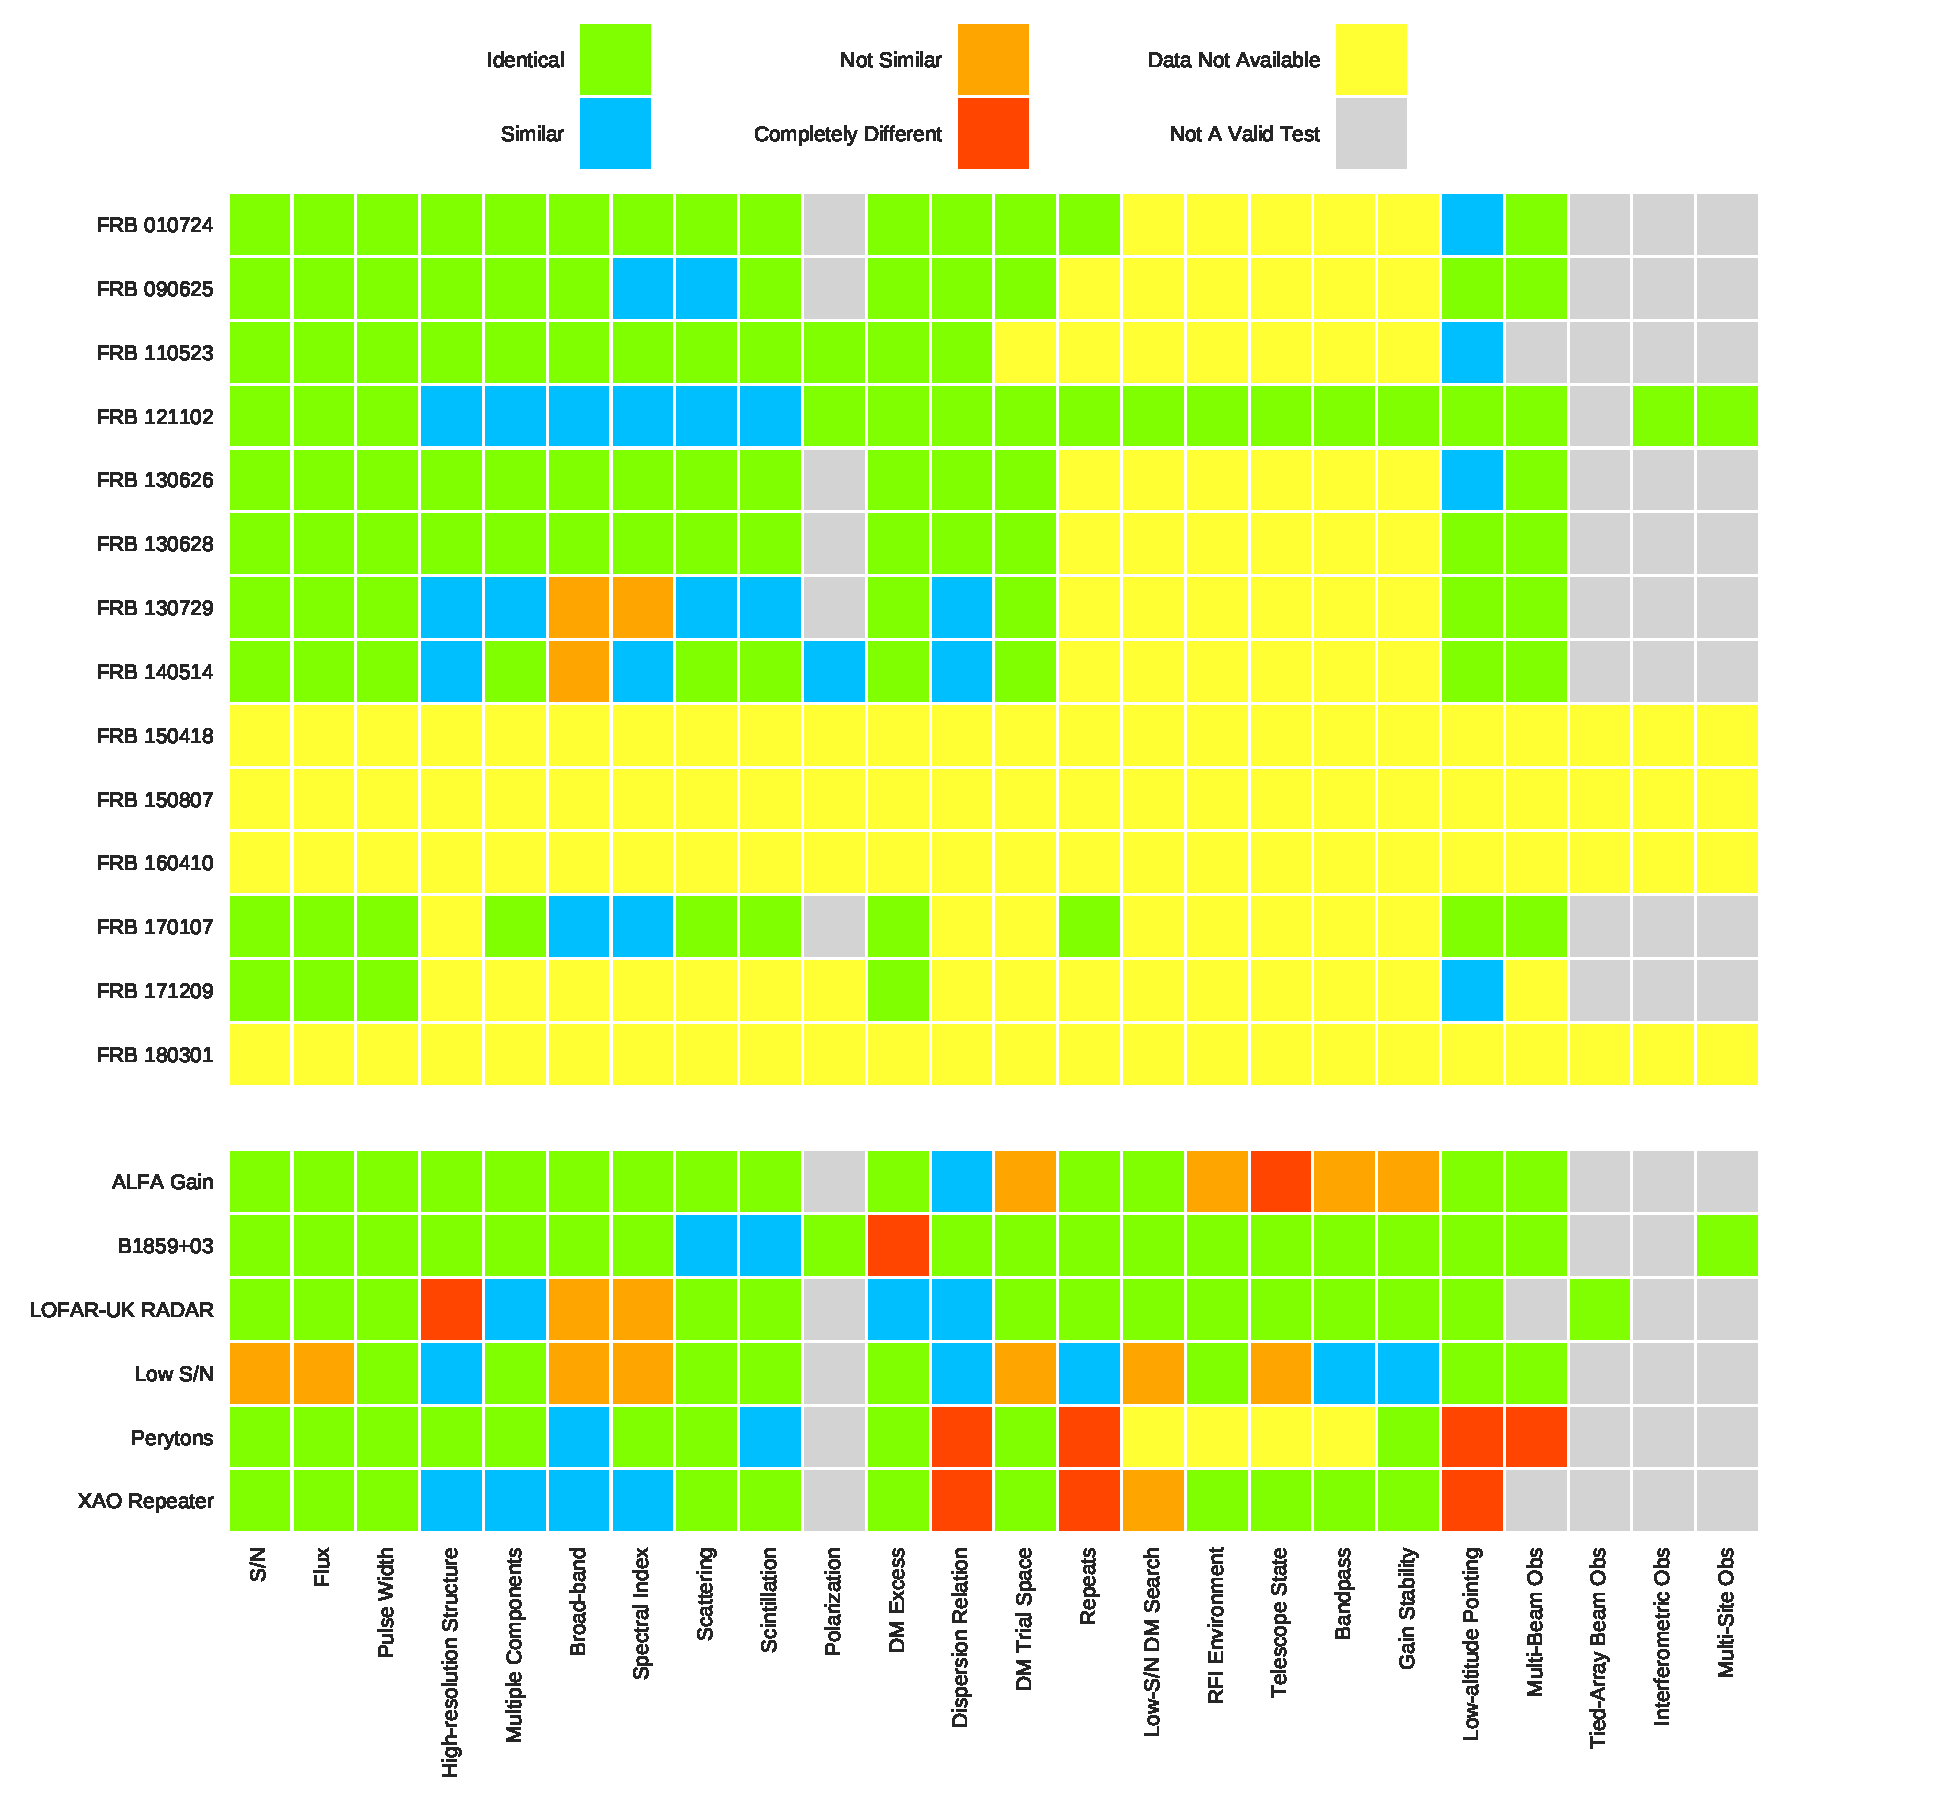
\includegraphics[width=1.0\linewidth]{verification/FRBheatmap.pdf}
    \caption{Verification criteria (Section \ref{sec:criteria}) heat map of some
    of the previously reported FRBs (top) and the terrestrial FRBs discussed in
    this work (bottom).  Green indicates a criterion test is identical to the
    prototypical detection or observation, thus providing evidence in favour of
    an astrophysical origin.  Blue indicates a criterion test result is similar
    to the prototype, but is not identical, and thus, is neutral evidence of an
    astrophysical origin.  Orange indicates the criterion results deviates from
    the expected prototype result and the event may be of terrestrial origin.
    Red indicates the criterion result is completely different from the
    prototype, and the event is terrestrial in origin. Yellow indicates the
    criterion result could not be determined from the available data.  Grey
    indicates the criteria is not valid based on the observation.
    }
    \label{fig:heat_map}
\end{figure*}

\subsection{FRB signals}

Having provided the FRB verification criteria above, we have re-analyzed the
previous reported \glspl{frb} based on the available literature and public data.
This analysis provides examples of answers 1-6 from Section \ref{sec:criteria}
for a number of sources. Figure \ref{fig:heat_map} captures the results in a
colour-coded table.  Overall, it is clear that the detections reported in the
literature score well against the prescribed criteria, which is to be expected
as many of these criteria are implicit to the observational definition of an
\gls{frb} such as high \gls{snr} and a line of sight dispersion measure in
excess of the Galactic contribution.

Starting from the lowest scores in our sampled set, we note that FRB130729 is
band-limited to the lower half of the observing band, and there is a sharp
decrease in flux around 1350~MHz (Figure \ref{fig:FRB130729}). We are using a
dispersion measure of 852~pc~cm$^{-3}$ which is different from the originally
reported dispersion measure of 861~pc~cm$^{-3}$. Using this new dispersion
measure there are two distinct components. The original detection paper
\citep{2016MNRAS.460L..30C} notes that FRB130729 is potentially due to
terrestrial \gls{rfi}, which is made clear in the low criteria scores.

% FRB130729
% aslxlap07:/local/griffin/data/FRB/FRB130729/FRB130729.ipynb
\begin{figure}
    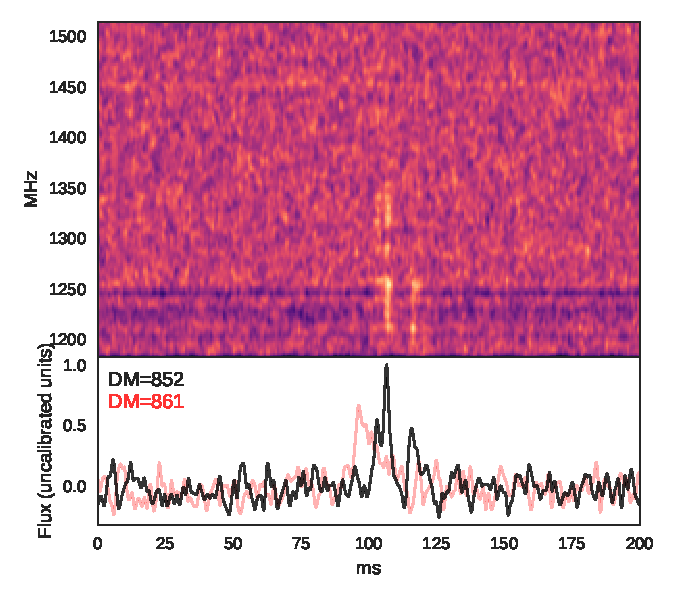
\includegraphics[width=1.0\linewidth]{figures/FRB130729.pdf}
    \caption{FRB130729 dedispersed with a DM of 852~pc~cm$^{-3}$ (black), this
    is different from the DM of 861~pc~cm$^{-3}$ (red) reported in
    \protect\cite{2016MNRAS.460L..30C}.  The detected FRB has two distinct
    components separated by approximately 10~ms. data are presented at the native
    recorded resolution of 64~$\mu$s, 390~kHz convolved with a Gaussian
    smoothing filter of size 512~$\mu$s, 3.125~MHz.}
    \label{fig:FRB130729}
\end{figure}

FRB140514 (Figure \ref{fig:FRB140514}) and FRB180301 (Figure
\ref{fig:FRB180301}) both score poorly in the broad-band criteria as the
majority of the detected flux is concentrated into narrow regions of the band.
This low score effects the dispersion relation criteria test as there is not
sufficient fractional bandwidth to perform a good fit. The frequency structure
of both of these detections could be due to scintillation. These low scores do
not discount FRB140514 and FRB180301 as astrophysical, they indicate that
FRB140514 and FRB180301 diverge from the prototypical \gls{frb} model.  We note
that FRB121102 diverges significantly from the prototype model as individual
pulses vary in bandwidth, apparent scattering, spectral index, and structure.
This is a useful example to show that the highest tests scores are not needed to
verify a detection as astrophysical.

% FRB140514
% aslxlap07:/local/griffin/data/FRB/FRB140514/FRB140514.ipynb
\begin{figure}
    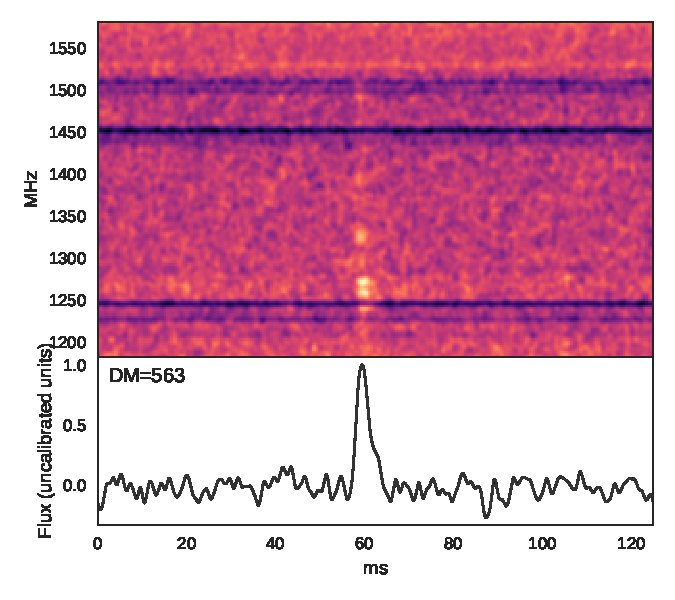
\includegraphics[width=1.0\linewidth]{figures/FRB140514.pdf}
    \caption{Dynamic spectrum of FRB140514 dedispersed with a DM of
    563~pc~cm$^{-3}$.  data are presented at the native recorded resolution of
    64~$\mu$s, 390~kHz convolved with a Gaussian smoothing filter of size
    512~$\mu$s, 3.125~MHz.
    }
    \label{fig:FRB140514}
\end{figure}

% FRB180301
% verification/verification_FRB180301.ipynb
\begin{figure}
    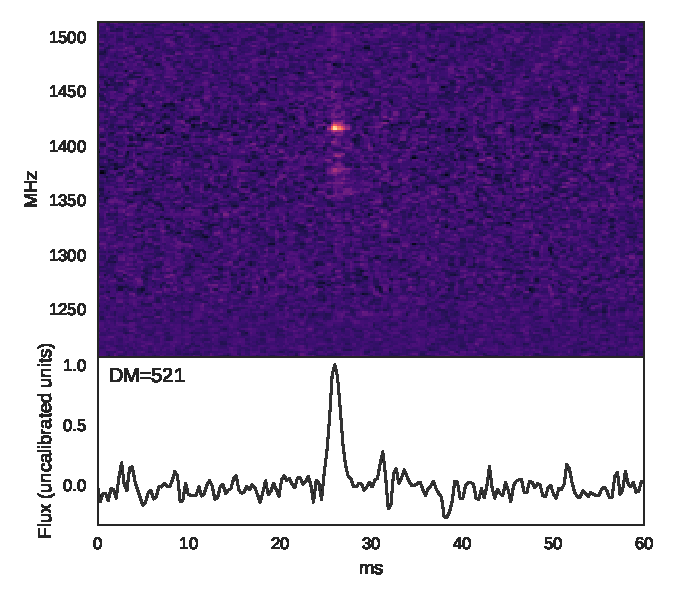
\includegraphics[width=1.0\linewidth]{figures/FRB180301.pdf}
    \caption{Dynamic spectrum of FRB180301 dedispersed with a DM of
    521~pc~cm$^{-3}$.  data are presented at the native recorded resolution of
    292.57~$\mu$s, 437.5~kHz convolved with a Gaussian smoothing filter of size
    29.2~$\mu$s, 875~kHz.
    }
    \label{fig:FRB180301}
\end{figure}

FRB010724 \citep{2007Sci...318..777L}, being the first reported detection, fits
the prototypical model well as many of the standard criteria we now use were
initially decided in the detection report.  Similarly, FRB110523, FRB130626, and
FRB130628 all well match the prototypical model, and thus show high scores in
most of the tests. FRB090625 shows variation in flux across the band, possibly
due to beam colorization or scintillation.  This is indicated by the lower
spectral index criteria score, but FRB090625 is otherwise also prototypical.
FRB150807 shows a drop in flux at the high end of the observing band due to a
steep apparent spectral index which is either intrinsic to the source or due to
the beam response. The reported detection included a number of system state
tests such as checking the gain and bandpass response, and the \gls{rfi}
environment which increases the overall scoring of this detection.

In most cases detections do not report on the telescope state and environment
during the time of detection. Though data are made public in many of the
detections, this data have all ready been normalized or calibrated so it is not
possible to verify the telescope state.  More recent detections are often
lacking in data or analysis. For example, very little information on FRB171209
has been reported, thus almost none of the criteria can be tested.  Providing
public data not only allow for independent verification, but also allow for
new tests to be run on previous detections.  For example, the lack of public
data of FRB170107 means that criteria not reported in the initial detection

%\subsubsection{FRB 110523}
%
%FRB 110523 is reported to have a magnetized plasma associated with the source.
%This conclusion was reached by detailed examination of the FRB parameters and
%comparisons to predicted parameters for its line of sight \cite{}.
%
%Using a dispersive delay fit which allows for the spectral index to vary, the
%authors find the delay to be proportional to $\nu^{-1.998}$  - a strong case for
%dispersion by a cold diffuse plasma. 
%
%The obtained DM value of 623.3 pc cm-3 is estimated to be almost 14 times the
%Galactic contribution, leading to a maximum redshift of 0.5 for the source.
%
%The authors also measure high fraction of linear polarization for this source of
%$\sim$ 44\%. The best RM fit to their data are $\sim$ -186.1 rad m$^{-2}$, much
%higher than the Galactic value of $\sim 18$ rad m$^{-2}$ that models predict for
%this line of sight.
%
%The RM estimate along with the scattering and scintillation estimates are
%checked against an observation of a known pulsar, B2319+60, less than 2 degrees
%away from the FRB position in the sky - using the same pipeline. The authors
%find that the pipeline estimates the RM of the pulsar correctly.
%
%The scintillation de-correlation bandwidth calculated for FRB110523 is found to
%be $\sim$1 MHz (i.e. a delay timescale of microseconds), comparable to the
%pulsar observation. This indicates that scintillation is likely due to the
%Galactic ISM.  
%
%The scattering observed through pulse broadening however, is much larger - on
%the order of milliseconds. This leads the authors to model the multipath
%propagation of the radio waves using two distinct scattering screens: one
%associated with the Milky Way and one close to the source. 
%
%(Scintillation should only occur if the first scattering screen is unresolved by
%the second.This allows them to estimate the host screen position)
%
%In their model the Galactic screen then produces micro-second scintillation
%while the host screen produce the larger millisecond scattering tail timescale.
%Best fit scattering spectral index is -3.6. 
%
%% scatter and scintil
%In the cases of e.g. FRB110523 and FRB170827, measurements of both scattering
%and scintillation have led to significant insights
%\citep{2015Natur.528..523M,2018arXiv180305697F}.  In both cases the $\tau$
%values, obtained through exponential fits to the broadened pulse shapes, were
%much larger than the timescales associated with the scintillation
%($\Delta\nu_d$) measurements. In the case of FRB110523, the $\Delta\nu_d$ value
%($\sim$1 MHz) was found to be similar to a nearby pulsar, suggesting that the
%scintillation is produced in the Milky Way. \cM{Strength of nearby pulsar to
%observe, make sure to mention elsewhere} The presence of two timescales lead to
%two-screen scattering models: a Galactic screen and a screen close to the FRB.
%Since scintillation will only be observed if the extra-galactic screen is
%sufficiently far away to be unresolved by the Galactic scattering surface, the
%authors concluded that FRB110523 is likely surrounded by a magnetized plasma. 
%
%Similarly, two distinct scattering timescales were calculated for FRB170827 and
%interpreted to be associated with 1) the Milky Way, and 2) either a host galaxy
%or the IGM. This FRB is the first to be discovered by the machine-learning
%detection algorithm implemented at the Molonglo Observatory Synthesis Radio
%Telescope (MOST). The system triggers voltage data capture (at the native time
%and frequency resolution), allowing for offline coherent dedispersion. \cM{This
%last info should possibly live somewhere else.}

\subsection{Terrestrial signals}

Also included in Figure \ref{fig:heat_map} are the results for the various
detections discussed in Section \ref{sec:false-pos}. We also include
PSR~B1859+03 as an example of single pulses from a pulsar during the ALFABURST
surveys.  In all these cases there is at least one failure.  The LOFAR RADAR
event shows artificial high-resolution structure.  Perytons and the XAO repeater
fail the dispersion relation test and repeat at different telescope pointings.
The ALFA gain variation has multiple negative test results relating to the
system response compared to the expected response.  The low \gls{snr} event does
not have a single critical test failure but fares poorly in several tests.  No
single test is sufficient to decide that an event is terrestrial. Figure
\ref{fig:heat_map} demonstrates how, given enough tests, a strong case can be
made to classify all these events as terrestrial.

\subsection{False-Positive Reporting}
During a search for anomalous signals we expect a number of reported false-positives events,
such as Perytons \citep{2011ApJ...727...18B} and the events presented in Section
\ref{sec:false-pos}. FRB130729 and FRB140514 have low scores on some of the
criteria tests, they do not fit the classic \gls{frb} model but given the
available observing and system information, and lack of an external,
anthropogenic explanation they are hard to discount as \textit{not} being of
astrophysical origin. It is necessary to report all of these events and to
provide as much evidence as possible to explain the origin of such events.

\section{Future Observational Methods}

Beyond detection of more \glspl{frb}, the goals of current surveys are to
localize the source to host galaxies, and detect pulses across broader
bandwidths and different frequencies in the radio spectrum. Verifiability should
also be considered in these surveys. This means capturing additional data as
discussed in Section \ref{sec:detect_report} and additional observing methods.

The simultaneous detection of signal with telescopes at multiple sites is
clear evidence for an astrophysical \gls{frb}.  Multi-site detectors, such as in
\gls{ligo}, are essential for false-positive rejection. Coordinating telescope
observations in logistically difficult, for example many FRB surveys run
commensally during targeted observations, but would prove invaluable in
reporting detections. Telescopes do not need to be observing at the same
frequency, only observing the same approximate field of view. Detection of an
event at multiple bands is strong evidence for an astrophysical source.

Localization with interferometric arrays produce similar results to a multi-site
observation. \gls{rfi} local to the site will still appear but it can be better
localized, and possibly determined to be in the near field. \gls{rfi} internal
to a single element would not correlate with other elements and would not appear
as a false-positive detection.  \gls{vlbi} detections provide the highest
confidence as the source is localized with multiple geographically isolated
telescopes.

Detection of \glspl{frb} at multiple frequencies not only adds to the scientific
understanding of the sources, but also help to verify that they are
astrophysical.  Due to historical development of receivers for pulsar searches,
most \glspl{frb} have been detected at L-band frequencies. Though, FRB110523
detected with the GBT and the multiple \glspl{frb} detected with UTMOST occurred
at UHF frequencies.  Only FRB121102 has been detected above L-band
\citep{atel10675}.  Such wide bands show the pulse structure goes beyond the
bandwidth of known source of \gls{rfi} (e.g. modulated RADAR). 

Multiple \glspl{frb} (e.g. FBR121102, FRB140514, FRB180301) have now been
detected which are not broad band, possibly due to the pulse progenitor,
lensing, or scintillation. It is likely that further narrow-band \glspl{frb}
exist is past survey data but do not pass the detection threshold. A pulse
search over subbands could reveal further detections as the \gls{snr} would
increase.

An ideal \gls{frb} search experiment would consist of at least three stations
geographically separated to reduce common \gls{rfi} and allow for localization.
Each station would consist of an aperture array or a compact array of
small-diameter/wide field of view elements. The effective bandwidth would be
sufficient to accurately determine a dispersion relation.  Coherent beams would
be formed across the primary beam. Each station would observe the same field.
Detections at multiple sites would then trigger a capture of the complex
voltages in a transient buffer which could then be correlated after the fact. 

Though this idealized experiment does not exist, it is currently possible to
make experiments that are close to it. LOFAR stations, though very low-frequency
compared to previous detections, can be configured to operate in a similar mode.
Telescopes that are part of \gls{vlbi} networks use the same back-ends and
contain complex voltage recorders can be used. Only a few telescopes in the
network that can have the same pointing are needed at a time.

\section{Conclusion}

From an observational point of view, \glspl{frb} are unique astronomical sources
as, so far, no follow-up observations have been able to verify a source using a
different telescope or observing frequency, except in the case of FRB121102
which is known to repeat. Thus, it is necessary to provide evidence for an
astrophysical origin when reporting a detection.

In Section \ref{sec:verify_crit} we have presented a set of criteria which can
be used to verify an \gls{frb} detection relative to a prototypical \gls{frb}
and observation. Some of the criteria are more essential to verification than
others.  For example, the strongest evidence for an event being of astrophysical
origin is a multi-site detection.  In combination these criteria become stronger
evidence for the origin of a detected \gls{frb}.

As the number of \gls{frb} surveys continues to increase in sensitivity, sampled
parameter space, and time, there will be an increase in the number of
false-positive detections, even as rejection models are improved.
Differentiating between true, astrophysical \glspl{frb} and false-positive
events will become more difficult.  Further, it could be that most astrophysical
\glspl{frb} are not prototypical as it is defined now, such as in the case of
FRB121102. Which indicate that some of the criteria must be relaxed,
making the differentiation more difficult still.  This should warrant the drive
towards interferometric and multi-site observations, complex-voltage data
recorders, subband pulse searches, and standard reporting of the observing
system.

Detection reporting incurs an economic cost in observing time, resources, and
human effort. Though, there is a scientific cost to delayed reporting as
follow-up observations could detect further pulses or multi-wavelength
observations could reveal an unknown counterpart to the radio pulse. An initial
detection will not be able to be verified against many of the criteria presented
here. But basic tests such as \gls{snr}, dispersion relation, and telescope
state can be automated to determine an initial detection `importance' in a
VO-Event trigger. This importance factor can then be adjusted accordingly as
more criteria are tested.

Reporting of false-positive events, even if the source is not explained, helps
to improve the robustness of search pipelines against systematics and \gls{rfi}.
Reporting these events also helps to improve the case for \glspl{frb} being of
astrophysical origin, just as the explanation for Perytons
\citep{2015MNRAS.451.3933P} removed doubt about detections using Parkes. An
attempt should be made to make the raw data, either unprocessed filterbank or
complex-voltage data, available to be used in independent verification and
testing on search pipelines.

Jupyter notebooks of the verification tests and terrestrial \glspl{frb} are
hosted on our public git
repository\footnote{https://github.com/griffinfoster/terrestrial-frb-letter}.

\bibliographystyle{mnras}
\bibliography{frb-detections} 

% Don't change these lines
\bsp	% typesetting comment
\label{lastpage}
\end{document}

% End of mnras_template.tex
